\RequirePackage[l2tabu,orthodox]{nag}

% \documentclass[headsepline,footsepline,footinclude=false,fontsize=11pt,paper=a4,listof=totoc,bibliography=totoc,BCOR=12mm,DIV=12]{scrbook} % two-sided % original source stated: BCOR=12mm,DIV=12
\documentclass[headsepline,footsepline,footinclude=false,oneside,fontsize=11pt,paper=a4,listof=totoc,bibliography=totoc,DIV=12]{scrbook} % one-sided

% TODO: change citation style in settings
\PassOptionsToPackage{table,svgnames,dvipsnames}{xcolor}

\usepackage[utf8]{inputenc}
\usepackage[T1]{fontenc}
\usepackage[sc]{mathpazo}
\usepackage[ngerman,english]{babel} % english is the same as american or USenglish
\usepackage[autostyle]{csquotes}
\usepackage[%
    backend=biber,
    url=true,
    style=numeric, % alphabetic, numeric
    sorting=none, % default == nty, https://tex.stackexchange.com/questions/51434/biblatex-citation-order
    maxnames=4,
    minnames=3,
    maxbibnames=99,
    giveninits,
    uniquename=init]{biblatex} % TODO: adapt citation style
\usepackage{graphicx}
\usepackage{scrhack} % necessary for listings package
\usepackage{listings}
\usepackage{lstautogobble}
\usepackage{tikz}
\usepackage{pgfplots}
\usepackage{pgfplotstable}
\usepackage{booktabs} % for better looking table creations, but bad with vertical lines by design (package creator despises vertical lines)
\usepackage[final]{microtype}
\usepackage{caption}
\usepackage[hidelinks]{hyperref} % hidelinks removes colored boxes around references and links
\usepackage{ifthen} % for comparison of the current language and changing of the thesis layout
\usepackage{pdftexcmds} % string compare to work with all engines
\usepackage{paralist} % for condensed enumerations or lists
\usepackage{subfig} % for having figures side by side
\usepackage{siunitx} % for physical accurate units and other numerical presentations
\usepackage{multirow} % makes it possible to have bigger cells over multiple rows in a table
\usepackage{array} % different options for table cell orientation
\usepackage{makecell} % allows nice manual configuration of cells with linebreaks in \thead and \makecell with alignments
\usepackage{pdfpages} % for including multiple pages of pdfs
\usepackage{adjustbox} % can center content wider than the \textwidth
\usepackage{tablefootnote} % for footnotes in tables as \tablefootnote
\usepackage{threeparttable} % another way to add footnotes as \tablenotes with \item [x] <your footnote> after setting \tnote{x} 

\usepackage{algorithm}
\usepackage{algorithmicx}
\usepackage{algpseudocode}
\usepackage{amsmath}
\usepackage{amsfonts}
\usepackage{tablefootnote}

\usepackage{svg}



\renewcommand{\algorithmicrequire}{\textbf{Input:}}
\renewcommand{\algorithmicensure}{\textbf{Output:}}

% https://tex.stackexchange.com/questions/42619/x-mark-to-match-checkmark
\usepackage{amssymb}% http://ctan.org/pkg/amssymb
\usepackage{pifont}% http://ctan.org/pkg/pifont
\newcommand{\cmark}{\ding{51}}%
\newcommand{\xmark}{\ding{55}}%


\usepackage[acronym,xindy,toc]{glossaries} % TODO: include "acronym" if glossary and acronym should be separated
\makeglossaries
\loadglsentries{pages/glossary.tex} % important update for glossaries, before document


\bibliography{bibliography}

\setkomafont{disposition}{\normalfont\bfseries} % use serif font for headings
\linespread{1.05} % adjust line spread for mathpazo font

% Add table of contents to PDF bookmarks
\BeforeTOCHead[toc]{{\cleardoublepage\pdfbookmark[0]{\contentsname}{toc}}}

% Define TUM corporate design colors
% Taken from http://portal.mytum.de/corporatedesign/index_print/vorlagen/index_farben
\definecolor{TUMBlue}{HTML}{0065BD}
\definecolor{TUMSecondaryBlue}{HTML}{005293}
\definecolor{TUMSecondaryBlue2}{HTML}{003359}
\definecolor{TUMBlack}{HTML}{000000}
\definecolor{TUMWhite}{HTML}{FFFFFF}
\definecolor{TUMDarkGray}{HTML}{333333}
\definecolor{TUMGray}{HTML}{808080}
\definecolor{TUMLightGray}{HTML}{CCCCC6}
\definecolor{TUMAccentGray}{HTML}{DAD7CB}
\definecolor{TUMAccentOrange}{HTML}{E37222}
\definecolor{TUMAccentGreen}{HTML}{A2AD00}
\definecolor{TUMAccentLightBlue}{HTML}{98C6EA}
\definecolor{TUMAccentBlue}{HTML}{64A0C8}

% Settings for pgfplots
\pgfplotsset{compat=newest}
\pgfplotsset{
    % For available color names, see http://www.latextemplates.com/svgnames-colors
    cycle list={TUMBlue\\TUMAccentOrange\\TUMAccentGreen\\TUMSecondaryBlue2\\TUMDarkGray\\},
}

% Settings for lstlistings

% Use this for basic highlighting
\lstset{%
    basicstyle=\ttfamily,
    columns=fullflexible,
    autogobble,
    keywordstyle=\bfseries\color{TUMBlue},
    stringstyle=\color{TUMAccentGreen}
}

% use this for C# highlighting
% %\setmonofont{Consolas} %to be used with XeLaTeX or LuaLaTeX
% \definecolor{bluekeywords}{rgb}{0,0,1}
% \definecolor{greencomments}{rgb}{0,0.5,0}
% \definecolor{redstrings}{rgb}{0.64,0.08,0.08}
% \definecolor{xmlcomments}{rgb}{0.5,0.5,0.5}
% \definecolor{types}{rgb}{0.17,0.57,0.68}

% \lstset{language=[Sharp]C,
% captionpos=b,
% %numbers=left, % numbering
% %numberstyle=\tiny, % small row numbers
% frame=lines, % above and underneath of listings is a line
% showspaces=false,
% showtabs=false,
% breaklines=true,
% showstringspaces=false,
% breakatwhitespace=true,
% escapeinside={(*@}{@*)},
% commentstyle=\color{greencomments},
% morekeywords={partial, var, value, get, set},
% keywordstyle=\color{bluekeywords},
% stringstyle=\color{redstrings},
% basicstyle=\ttfamily\small,
% }

% Settings for search order of pictures
\graphicspath{
    {logos/}
        {figures/}
}

% Set up hyphenation rules for the language package when mistakes happen
\babelhyphenation[english]{
    an-oth-er
    ex-am-ple
}

% Decide between
%\newcommand{\todo}[1]{\textbf{\textsc{\textcolor{TUMAccentOrange}{(TODO: #1)}}}} % for one paragraph, otherwise error!
%\newcommand{\done}[1]{\textit{\textsc{\textcolor{TUMAccentBlue}{(Done: #1)}}}} % for one paragraph, otherwise error!
% and
\newcommand{\todo}[1]{{\bfseries{\scshape{\color{TUMAccentOrange}[(TODO: #1)]}}}} % for multiple paragraphs
\newcommand{\done}[1]{{\itshape{\scshape{\color{TUMAccentBlue}[(Done: #1)]}}}} % for multiple paragraphs
% for error handling of intended behavior in your latex documents.

\newcommand{\tabitem}{~~\llap{\textbullet}~~}

\newcolumntype{P}[1]{>{\centering\arraybackslash}p{#1}} % for horizontal alignment with limited column width
\newcolumntype{M}[1]{>{\centering\arraybackslash}m{#1}} % for horizontal and vertical alignment with limited column width
\newcolumntype{L}[1]{>{\raggedright\arraybackslash}m{#1}} % for vertical alignment left with limited column width
\newcolumntype{R}[1]{>{\raggedleft\arraybackslash}m{#1}} % for vertical alignment right with limited column width

\newcommand*{\getUniversity}{Technische Universität München}
\newcommand*{\getFaculty}{Department of Informatics}
\newcommand*{\getTitle}{LiDAR and camera data fusion for the biologically inspired SLAM systems}
\newcommand*{\getTitleGer}{LiDAR und Kameradaten Fusion für die biologisch inspirierten SLAM-Systeme}
\newcommand*{\getAuthor}{Jakub Šťastný} 
\newcommand*{\getDoctype}{Bachelor's Thesis in Informatics}
\newcommand*{\getSupervisor}{Prof. Dr.-Ing. habil. Alois C. Knoll}
\newcommand*{\getAdvisor}{Genghang Zhuang, M.Eng.}
\newcommand*{\getSubmissionDate}{15.09.2022} % TODO check date format
\newcommand*{\getSubmissionLocation}{Munich}

\begin{document}

\selectlanguage{english}

\pagenumbering{alph}
\begin{titlepage}
  % HACK for two-sided documents: ignore binding correction for cover page.
  % Adapted from Markus Kohm's KOMA-Script titlepage=firstiscover handling.
  % See http://mirrors.ctan.org/macros/latex/contrib/koma-script/scrkernel-title.dtx,
  % \maketitle macro.
  \oddsidemargin=\evensidemargin\relax
  \textwidth=\dimexpr\paperwidth-2\evensidemargin-2in\relax
  \hsize=\textwidth\relax

  \centering

  \IfFileExists{logos/tum.pdf}{%
    
\includegraphics[height=20mm]{logos/tum.pdf}
  }{%
    \vspace*{20mm}
  }

  \vspace{5mm}
  {\huge\MakeUppercase{\getFaculty{}}}\\

  \vspace{5mm}
  {\large\MakeUppercase{\getUniversity{}}}\\

  \vspace{20mm}
  {\Large \getDoctype{}}

  \vspace{15mm}
  \makeatletter
  \ifthenelse{\pdf@strcmp{\languagename}{english}=0}
  {\huge\bfseries \getTitle{}}
  {\huge\bfseries \getTitleGer{}}
  \makeatother

  \vspace{15mm}
  {\LARGE \getAuthor{}}

  \IfFileExists{logos/faculty.png}{%
    \vfill{}
    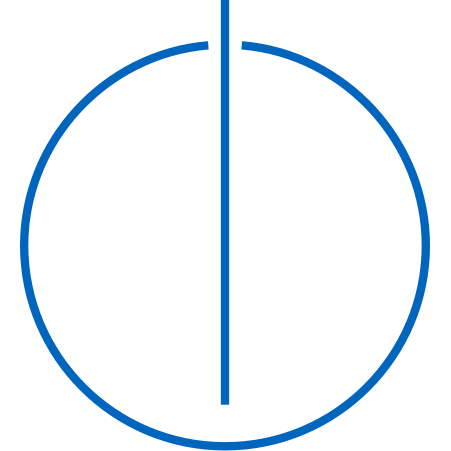
\includegraphics[height=20mm]{logos/faculty.png}
  }{}
\end{titlepage}

\frontmatter{}
\begin{titlepage}
  \centering

  \IfFileExists{logos/tum.pdf}{%
    
\includegraphics[height=20mm]{logos/tum.pdf}
  }{%
    \vspace*{20mm}
  }

  \vspace{5mm}
  {\huge\MakeUppercase{\getFaculty{}}}\\

  \vspace{5mm}
  {\large\MakeUppercase{\getUniversity{}}}\\

  \vspace{20mm}
  {\Large \getDoctype{}}

  \makeatletter
  \vspace{15mm}
  \ifthenelse{\pdf@strcmp{\languagename}{english}=0}
  {
  {\huge\bfseries \getTitle{}}

  \vspace{10mm}
  {\huge\bfseries \foreignlanguage{ngerman}{\getTitleGer{}}}
  }
  {
  {\huge\bfseries \getTitleGer{}}

  \vspace{10mm}
  {\huge\bfseries \foreignlanguage{english}{\getTitle{}}}
  }
  \makeatother

  \vspace{15mm}
  \begin{tabular}{l l}
    Author:          & \getAuthor{} \\
    Supervisor:      & \getSupervisor{} \\
    Advisor:         & \getAdvisor{} \\
    Submission Date: & \getSubmissionDate{} \\
  \end{tabular}

  \IfFileExists{logos/faculty.png}{%
    \vfill{}
    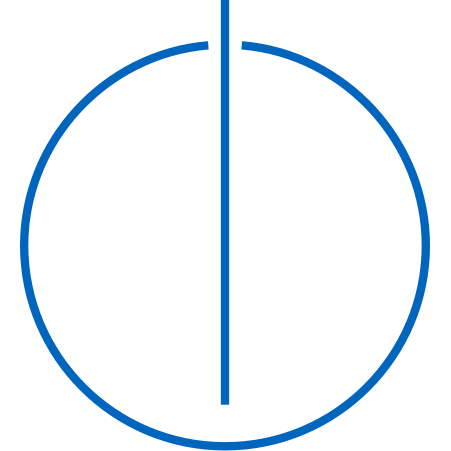
\includegraphics[height=20mm]{logos/faculty.png}
  }{}
\end{titlepage}

\cleardoublepage{}

\thispagestyle{empty}
\vspace*{0.8\textheight}
\noindent
\makeatletter
\ifthenelse{\pdf@strcmp{\languagename}{english}=0}
{I confirm that this \MakeLowercase{\getDoctype{}} is my own work and I have documented all sources and material used.}
{Ich versichere, dass ich diese \getDoctype{} selbstständig verfasst und nur die angegebenen Quellen und Hilfsmittel verwendet habe.}
\makeatother

\vspace{15mm}
\noindent
\getSubmissionLocation{}, \getSubmissionDate{} \hspace{50mm} \getAuthor{}

\cleardoublepage{}

% \makeatletter
\ifthenelse{\pdf@strcmp{\languagename}{english}=0}
{\addcontentsline{toc}{chapter}{Acknowledgments}}
{\addcontentsline{toc}{chapter}{Danksagungen}}
\makeatother
\thispagestyle{empty}

\vspace*{20mm}

\begin{center}
\makeatletter
\ifthenelse{\pdf@strcmp{\languagename}{english}=0}
{\usekomafont{section} Acknowledgments}
{\usekomafont{section} Danksagungen}
\makeatother
\end{center}

\vspace{10mm}

%TODO: Acknowledgments

\cleardoublepage{}

\chapter{\abstractname}

Simultaneous localization and mapping is a crucial problem for most autonomous mobile robots. RatSLAM is a biologically inspired SLAM system that simulates the rodent's brain using the Pose Cell network, odometry, and visual input. This system demonstrates long-term stability and accurate results in indoor and outdoor environments. One of the essential parts of RatSLAM is a scene recognition algorithm. Whereas RatSLAM uses a visual scene recognition approach, this work suggests a technique to combine data from 3D LiDAR and camera to achieve better scene recognition results and hence improve the whole SLAM system. Compared to the camera, the LiDAR sensor is more accurate and robust to changing light conditions. This thesis proposes several scene recognition approaches using combined data from the camera and 3D LiDAR sensor. These approaches are combined with RatSLAM to build an improved biologically inspired SLAM system. All proposed methods are tested on performance using several evaluation metrics and compared with visual scene recognition and OpenRatSLAM. As the results show, the suggested methods are capable of accurate and robust scene recognition, and final SLAM systems are able to construct suitable experience maps. Furthermore, all proposed approaches outperformed the OpenRatSLAM in most of the evaluated metrics and worked smoothly also in situations where OpenRatSLAM failed.


\makeatletter
\ifthenelse{\pdf@strcmp{\languagename}{english}=0}
{\renewcommand{\abstractname}{Kurzfassung}}
{\renewcommand{\abstractname}{Abstract}}
\makeatother

\chapter{\abstractname}

\begin{otherlanguage}{ngerman}

    Simultaneous localization and mapping ist ein entscheidendes Problem für die meisten autonomen mobilen Roboter. RatSLAM ist ein biologisch inspiriertes SLAM-System, das das Gehirn des Nagetiers mithilfe des Pose Cell-Netzwerks, Odometrie und visueller Eingabe simuliert. Dieses System zeigt langfristige Stabilität und genaue Ergebnisse in Innen- und Außenumgebungen. Einer der wesentlichen Bestandteile von RatSLAM ist ein Szenenerkennungsalgorithmus. Während RatSLAM einen visuellen Szenenerkennungsansatz verwendet, schlägt diese Arbeit eine Technik vor, um Daten von 3D-LiDAR und Kamera zu kombinieren, um bessere Ergebnisse bei der Szenenerkennung zu erzielen und somit das gesamte SLAM-System zu verbessern. Im Vergleich zur Kamera ist der LiDAR-Sensor genauer und robuster gegenüber wechselnden Lichtverhältnissen. Diese Arbeit schlägt mehrere Ansätze zur Szenenerkennung vor, die kombinierte Daten von der Kamera und dem 3D-LiDAR-Sensor verwenden. Diese Ansätze werden mit RatSLAM kombiniert, um ein verbessertes biologisch inspiriertes SLAM-System aufzubauen. Alle vorgeschlagenen Methoden werden anhand mehrerer Bewertungsmetriken auf ihre Leistung getestet und mit visueller Szenenerkennung und OpenRatSLAM verglichen. Wie die Ergebnisse zeigen, sind die vorgeschlagenen Verfahren zu einer genauen und robusten Szenenerkennung in der Lage, und endgültige SLAM-Systeme sind in der Lage, geeignete Erfahrungskarten zu erstellen. Darüber hinaus übertrafen alle vorgeschlagenen Ansätze OpenRatSLAM in den meisten der bewerteten Metriken und funktionierten reibungslos auch in Situationen, in denen OpenRatSLAM versagt hat.

\end{otherlanguage}


\makeatletter
\ifthenelse{\pdf@strcmp{\languagename}{english}=0}
{\renewcommand{\abstractname}{Abstract}}
{\renewcommand{\abstractname}{Kurzfassung}}
\makeatother

\microtypesetup{protrusion=false}
\tableofcontents{}
\microtypesetup{protrusion=true}

\mainmatter{}

\chapter{Introduction}\label{chapter:introduction}

Nowadays, mobile robots are becoming more and more popular. Whether it is an autonomous car, a transport robot in a warehouse, or an automatic vacuum cleaner, these robots are finding more and more applications and becoming a part of most people's everyday lives.\par
One of the essential tasks every mobile robot must be able to solve is finding a valid path from its current position to the target based on the obstacles and surroundings. Knowledge of the robot's precise location and environment map is a necessary prerequisite for almost any navigation and planning algorithm.\par
Even if most of the world is already mapped on a large scale and due to GPS, Gallileo, GNSS, etc., we can locate ourselves on these maps with satisfiable accuracy, these methods can not be usually used for the indoors or small scale environments, where the maps are typically unknown, and any global positioning services can not be used.\par
Furthermore, a proper self-localization of the robot depends on a precise map, and map construction depends on the accurate positions of a robot and other landmarks. Therefore the localization and mapping problems have to be usually solved simultaneously. In addition, the environment can frequently change, which makes, together with the mutual dependence of localization and mapping, the simultaneous localization and mapping (SLAM) a very challenging problem, that most mobile robots must solve.\par
The SLAM has been solved by many scientists since the 1980s. Until now, there have been developed many different techniques for solving the SLAM, with various advantages and disadvantages. The majority of the approaches can be separated into three main categories: conventional SLAM, visual SLAM, and biologically inspired SLAM.\par
The conventional algorithms are based on a probabilistic model and usually work with Light Detection And Ranging \cite{LiDar} and odometry sensors. These techniques typically work in two steps. In the first step, the position of the robot and landmarks are extracted from the raw sensor data, usually using different filtering techniques, such as Kalman filter or particle filtering. This extracted information is used in the second step to build or update the final map.\cite{convSLAM}\par
The precision and resolution of the final maps built by these approaches are usually very high. However, there is usually a high computation and storage demand that rapidly increases with the number of landmarks. Because of this fact, the conventional techniques are generally not suitable for larger or complicated environments with a lot of landmarks and can not be performed on low-performance computation devices, such as older Raspberry PI models. Furthermore, many of these techniques usually rely on accurate sensor measurements and are not robust against more significant measurement errors that can easily destroy the whole map.\par
The visual SLAM approaches became popular mostly during the last decade, with cameras' significant cost reduction and quality improvement. As the name suggests, these techniques are based on visual input from a 2D or 3D camera and various computer vision techniques. Compared to conventional methods, these approaches obtain more information about the environment and, therefore, can generate more precise outputs. However, most visual SLAM methods are susceptible to ambient lighting and reflections and perform differently in different light conditions, which can cause significant errors. Furthermore, these techniques work poorly in a low-texture environment, making them unsuitable for environments with many windows, mirrors, or other glass or reflective surfaces.\cite{visualSLAM}\par
As the name suggests, the biologically inspired SLAM approaches find their inspiration in various biological systems. The ideas behind these techniques are very diverse and differ from approach to approach. In this category, we include techniques based on machine learning, models of biological structures, or methods based on the behavior of some biological species. These techniques usually can not guarantee the result's precision but use a heuristic approach to approximate the results with specified accuracies. These techniques generally have a significantly lower demand for resources than conventional and visual approaches. Furthermore, these techniques are usually more robust against measurement errors and can also contain a mechanism to repair the previous errors based on the new data.\par
One of the most generally known biologically inspired SLAM systems is RatSALM, which was initially developed in 2008 and improved over the years \cite{RatSLAM}. The open source version of this technique, the OpenRatSLAM \cite{OpenRatSLAM}, and its ROS implementation RatSLAMRos \cite{RatSLAMROS} brings a standardized, reconfigurable, and modulized way to include this method to any program for mobile robots. Furthermore, the RatSLAM approach shows long-term stability in the indoors and outdoors scenarios.\cite{RatSLAMExp1}\cite{RatSLAMExp2}\cite{RatSLAMExp3}\cite{RatSLAMExp4}\par
This approach is inspired by computational models of the hippocampus of rodents, which have been extensively studied concerning navigation tasks and show many of the properties of a desirable SLAM solution. During the last 50 years, four essential kinds of neurons have been discovered connected with SLAM and navigation tasks: place cells, grid cells, head direction cells, and border cells.\par
Place cells, discovered by John O'Keefe in 1976 \cite{placeCells}, are connected with different places the rodent has visited and are activated every time the rat returns to a particular location. Grid cells, discovered by Edvard and May-Britt Moser in 2008 \cite{gridCells}, react to the rodent's movement and are activated in sequence as the rat moves around in the environment. The head direction cells allow the rodent to get the spatial sense of direction based on geometry features. Finally, the border cells are activated when the rodent moves close to a wall or other obstacle.\par
According to biological inspiration, localization is based on odometry, inspired by the Grid cells. Odometry is well known for its problems with cumulative errors. It does not matter how precise odometry sensors or techniques are used; even a very small error adds up over time, and the whole system will be completely out of reality after a few minutes, maximally a few hours. To reduce these errors, a loop closure technique is required. Based on the biological model, the RatSLAM implements the loop closure using a place recognition technique.\par
So, place recognition is one of the crucial parts of the RatSLAM solution and any intelligent system operating autonomously over a longer period of time. The main task of this problem is to tell if the robot has visited the current place before or not, despite several changes in its appearance due to different light conditions, weather, or non-stationary objects like pedestrians or cars.\par
Most standard place recognition techniques are based on visual input and usually use machine learning, feature extraction and matching, or the scene decomposition approaches. However, some other methods exist based on entirely different ideas and kinds of sensors.


\section{Motivation}\label{section:motivation}

The original RatSLAM approach uses a low-resolution camera image as an input for place recognition. However, as mentioned before, this brings some drawbacks, like sensitivity to the different light conditions and reflections. Compared to a camera, a 3D LiDAR sensor can measure directly in three dimensions with a high precision, even over a long distance. Furthermore, the 3D-LiDAR sensor is robust against different light conditions and reflections. On the other hand, compared to the camera, the LiDAR data lose some helpful information, like colors, that can be a critical factor in place recognition of places in the environments like office buildings with different meeting rooms that differ only in the wall color and otherwise remain identical.\par
The proper combination of the advantages of both these sensors can significantly improve place recognition and consequently enhance the quality of the entire RatSLAM algorithm. Furthermore, the additional odometry sensor may provide more accurate speed data, improving the SLAM quality compared to the original RatSLAM, which calculates odometry information only from the visual input.\par
Lastly, place recognition based on visual data requires storing whole images or extracted feature vectors, which consumes a relatively large amount of memory. The proper representation of the scene based on the LiDAR and camera data may significantly improve the required space and make RatSLAM even more suitable for the low performant computational devices.

\section{Objectives}\label{section:objectives}

This thesis aims to find an optimal method of combining data from several sensors and find the best solution for the place recognition problem and, as a result, improve the precision and performance of the RatSLAM algorithm. Besides, all suggested approaches find inspiration in biological systems, like the rest of the RatSLAM approach.\par
To achieve this primary goal, several challenges need to be solved. The first challenge is data fusion. In this part, the optimal scene representation must be designed to combine most of the information from all the sensors and reduce most of the disturbing factors typical for the input sensors. Furthermore, the synchronization and mutual calibration of the sensor must be solved.\par
The other challenge is to solve the place recognition problem based on the representation from the fused data. In this part, we need to think apart from accuracy to the performance and memory consumption in order to make this approach available for low-performance devices.\par
There will be suggested several algorithms with different expected advantages and disadvantages. All proposed techniques will be tested on accuracy and various performance metrics and compared to each other, as well as to an image-based place recognition used in an original RatSLAM.

\section{Work Contribution}\label{section:workContribution}

First, I came up with a compact scene representation that combines the advantages of both LiDAR and the camera. Then I suggested a practical approach to fuse the data received from the sensors into the chosen representation. This part also contained sensor synchronization and calibration.\par
Afterward, I designed a compact and suitable scene template that will be stored in the memory. While creating the template, I followed the biological inspiration, namely the model of human spatial memory. I also devised a method to extract the designed template from the fused scene representation effectively. Finally, after preparing the template model, I created an approach to compare two of these templates and thus solved the scene recognition problem.\par
The suggested algorithm was based on scene decomposition, object detection, and extraction of the significant properties of each object. However, this approach did not consider the objects' exact shape, leading to a considerable increase of false positive evaluations in several environments. To eliminate these false positive evaluations, I came up with a 2 stage approach. This approach was based on the originally designed method. All scenes were evaluated same as before; however, all positive evaluations were re-evaluated using a neural network in the second stage.\par
To create a working second stage, I choose suitable network architecture and experimentally found the best network's dimensions. After deciding on the network architecture, I made appropriate training datasets and trained and tested the model.\par
The suggested approach was dependent on many different parameters. The optimal parameters had to be found to maximize the place recognition performance. So, I came up with an optimization method that finds an optimal parameters vector, maximizing the approach's accuracy. In order to implement this optimization method, I created a set of tools for manual and automatic performance testing and analysis.\par
After the scene recognition algorithm was finished, I successfully integrated it with RatSLAM and created a robust biologically inspired SLAM system. I made the whole system in ROS to ensure its modularity, reconfigurability, reusability, and easy improvement.\par
After creating the whole system, I devised several evaluation metrics to test all critical methods' properties. I set up a robust testing simulation in several environments and created reusable testing datasets to ensure the reproducibility of all experiments. Finally, I tested all suggested techniques and the OpenRatSLAM approach, found an appropriate presentation of the results, and compared all presented methods.

\section{Outline}\label{section:outline}

\textbf{Chapter 2} presents a related work about various scene recognition approaches and biologically inspired SLAM systems.\\
\textbf{Chapter 3} describes all frameworks and tools used in this work.\\
\textbf{Chapter 4} provides a detailed description of all the algorithms and techniques implemented in this thesis. Namely, the complete system overview is provided in the beginning, followed by the solution to the data fusion problem. Afterward, three different place recognition techniques are offered.\\
\textbf{Chapter 5} evaluates the performance of approaches presented in chapter 4 and compares them with the OpenRatSLAM. The beginning of the chapter introduces the test environments and evaluation metrics. The following four sections will discuss the results of the different evaluation metrics. In the penultimate section will be tested the integration of the place recognition approaches with RatSLAM. Finally, the last section summarizes all measured results and discusses all suggested techniques' final performance and advantages or disadvantages.\\
\textbf{Chapter 6} summarizes the whole work, alerts to possible drawbacks, and suggests future work.\\

\chapter{Related Work}\label{chapter:relatedWork}

\section{Scene recognition problem}\label{section:sceneRecognitionProblem}

Scene recognition is a problem that received a lot of attention from many researchers and engineers in the last few years. Even if approaches for several sensors were developed, the most popular is visual scene recognition based on images from a camera.\par
This section presents some of the most popular approaches for visual scene recognition based on traditional methods and machine learning.

\subsection{Local image descriptors}\label{section:localImageDescriptors}

This technique aims to find, describe and compare significant features from the images. Each image is processed in two phases: detection and description. Since both stages can be solved independently, a large number of various approaches for each phase have been developed.\par
The detection phase aims to detect all essential features in a given image, such as edges, corners, significant points, or objects. The feature detection algorithms generate pixel coordinates of each feature, usually with an occupied area. There are many different approaches to this problem, like FAST \parencite{FAST}, Laplacian of Gaussian \parencite{LaplacianOfGaussian}, SUSAN \parencite{SUSAN}, and many more, detecting different kinds of features.\par

TODO image of feature detection example

The goal of the description phase is to provide a summary of the image information around each feature. The feature is represented as its position in the image, and the output is defined as an N-dimensional vector. A good feature descriptor should fulfill three following rules: Repeatability, Distinctiveness, and Efficiency. The repeatability means that the feature descriptor is robust and invariant to the image's translation, rotation, or illumination changes. Distinctiveness represents the ability to distinguish between two close features. Finally, due to real-time processing, which is increasingly applied nowadays, efficiency also plays an important role. Among popular approaches to solve this problem can be included SURF \parencite{SURF}, GLOH \parencite{GLOH}, BRIEF \parencite{BRIEF}, and many more.\par
Using these two stages, the set of local image descriptors
$$
    \mathbf{X} = [\mathbf{x}_0, \mathbf{x}_1, \dots, \mathbf{x}_{n-1}]^T
$$
is extracted, in which $\textbf{x}_i \in \mathbb{R}^k$. However, each image can contain hundreds of individual features, which can be impractical in real-time processing and requires a huge amount of memory. To lower the dimensions of the local descriptors vector, different techniques like bag-of-visual-words \parencite{BagOfVisualWords1}\parencite{BagOfVisualWords2}, VLAD \parencite{VLAD}, or Fisher kernel \parencite{FisherKernel} may be applied to aggregate the vector $\mathbb{X}$ into a more compact single vector. Finally, these vectors are compared to decide if two images represent the same place. The precise comparison technique depends on the techniques used in the description phase and for the final descriptors' vector compression.

\subsection{Global image descriptors}\label{section:globalImageDescriptors}

This technique works similarly to the previous one, with one big difference. In this approach, the detection phase is wholly omitted, and the whole image is considered as only one feature. Therefore, the feature description algorithms must be modified to suitably describe large and diverse features. Some alternations of the algorithms provided in the last part might be WI\_SURF \parencite{WiSurf} or BRIEF-GIST \parencite{BRIEFGIST}.

\subsection{Neural networks based approaches}\label{section:neuralNetworksBasedApproaches}

Convolutional neural networks achieve outstanding performance on several recognition or classification tasks, including a solution to scene recognition problems \parencite{CNNSceneRecognition1} \parencite{CNNSceneRecognition2}. The basic idea behind this approach is similar to the presently presented technique. In the first step, the global feature descriptor is extracted from the image and afterward compared with the other extracted feature vectors. However, unlike the previously presented technique, this approach uses machine learning instead of classical techniques to perform these two tasks.\par
According to the studies \cite{fischer2014descriptor}\cite{Imagenet}, the features extracted from images using convolutional neural networks significantly outperform the features extracted by classical algorithms like SIFT. There are many different kinds of convolutional neural networks used for these purposes. From the most popular ones, we can mention VGGNet \parencite{VggNet} or GoogleNet \parencite{GoogleNet}.

\section{Biologically inspired SLAM systems}\label{section:bioSlam}

\subsection{RatSLAM}\label{section:ratSlamRW}

\subsection{Other RatSLAM variants}\label{section:ratSlamVariants}
\chapter{Technical Background}\label{chapter:technicalBackground}

This chapter provides an overview of most of the techniques, frameworks, and libraries related to the thesis, including the Robot Operating System ROS, used Lidar sensors, Gazebo, Turtlebo3 models, RViz, OpenCV, Pytorch, PointNet, and different models used for the representation of colors and calculating of their differences.

\section{Robot Operating System}\label{section:ROS}

Robot Operating System\cite{ros}, shortly ROS is a popular open-source framework commonly used by many researchers and robot developers. This framework allows easy launch, deployment, and communication between different modules as standalone services that create a final complex system. This modularity permitted the creation and easy application of various tools and libraries like Gazebo, RViz, or rqt, together with custom services. Furthermore, the ROS allows an easy spread of one system among more devices, allowing an easy run of some services directly on the robot and other services on the central computer, without almost any accessive work.\par
Another significant advantage of the ROS's modularity is that you can exchange the robot simulator with the real robot and sensors without touching the rest of the system. Furthermore, you can record and replay the entire system's messages during its run, allowing easy reproducibility of any experiment.\par
The official languages of the ROS are C++ and Python, but there are also inofficial tools that allow writing services for ROS in other languages, like, for example, LISP \cite{RosLISP} or Swift\cite{RosSwift}.\par
The following subsections briefly introduce some of the essential ROS features.

\subsection*{Roscore}

Roscore is a service that must be executed before running any Node of the ROS system. This service will automatically start all the essential services for the ROS running, like logging service, parameter server, and ROS master. Therefore, the running roscore service is necessary for ROS nodes to communicate.

\subsection*{ROS Node}

Ros Nodes are a crucial concept of the whole system. Single Node represents a standalone service that can process data received from other ROS Nodes, sensors, or users and send them to the other Nodes or directly to the user or system actors. The entire application usually consists of many ROS Nodes that communicate using ROS topics, services, etc.

\subsection*{ROS message}

Messages are the most common way of communication between several ROS Nodes. These messages are transmitted between the Nods via ROS topics. The ROS message, typically stored in the .msg file, describes a format that the data transmitted on a particular ROS topic must fulfill and tells the ROS Node how to represent the received data.\par
According to the convention, most messages start with the Header part, containing the message sequence number, timestamp, and frame id. However, this header is optional and is not present in all commonly used messages.

\subsection*{ROS topic}

ROS topics are named buses, serving for message exchange between the Nodes. One or more Nodes can publish messages or subscribe to each ROS topic and receive all published messages. The publishing and subscribing processes work anonymously, which means that the publisher does not know if the message was read by only one or more or any Node, and receivers do not know which node published the particular message unless it's part of the sent data.\par
Every topic is strongly connected with a particular message type, so every message published on the same topic must have the same format.

\subsection*{Roslaunch}

Roslaunch is a tool allowing the launch of multiple ROS Nodes with a single command based on an XML configuration. This tool also supports setting different parameters that can be set while starting the process and passed to the particular Nodes or put on the Parameter Server. Furthermore, this tool allows renaming specified topics without the need to tell any information to the publishing Nodes.

\subsection*{ROS package}

ROS packages help to organize the ROS software. The package can contain ROS Nodes, libraries, datasets, configuration files, etc. The goal of the ROS package is to pack together connected ROS Nodes and other tools that together create some meaningful tool, program, or library. These packages allow easy publication, deployment, installation, and integration of the third-party components into custom programs or systems.

\subsection*{Rosbag}

Rosbag is a command line tool for recording and replaying the data exchanged between Nodes during the program run. This tool can record all messages published on all or only specified ROS topics without affecting the running system. These messages can be later replayed, which allows excellent reproducibility of all program runs and further optimization, improvement, and testing under the same conditions.\par
Particularly researchers with this tool record all data from the sensors while running experiments and publish them on the internet for later experiment reproduction or further development.

\subsection*{Catkin}

Catkin is a collection of CMake macros and Python scripts commonly used for the ROS development and building of ROS Nodes and packages. Even if catkin is not the official part of ROS, it is a widely used tool among the ROS community.

\section{Gazebo}\label{section:gazebo}

Gazebo is a famous open-source 3D-simulation tool supporting robot simulation in complex 3D environments, including realistic physics, like gravity, friction, collisions, light reflections, etc. These environments can also change over time, which allows adding pedestrians, moving cars, or other non-stationary objects to the simulation.\par
Furthermore, Gazebo supports various types of sensors, especially HD-Camera, 3D or 2D Lidar, IMU, etc., or several plugins for the robot control. This tool also provides an interface fully compatible with ROS, which makes it a perfect simulation tool for this thesis.

\section{Turtlebot3}\label{section:turtlebot}

Turtlebot3 offers open-source mobile robots commonly used in robotics research and development. The Turtlebo3 provides two different models, Burger and Waffle-Pi, that are fully compatible with the Gazebo simulator and contain all software necessary for the robot control and simulation. These models are also easily extensible and allow adding new kinds of sensors.

\section{RViz}\label{section:rviz}

RViz is a ROS graphical interface, allowing the visualization of the information published for many different available topics. Particularly, this tool is commonly used for the real-time visualization of the data received from various sensors, generated maps, landmarks, detected objects, etc.

\section{OpenCV}\label{section:openCv}

OpenCV\cite{OpenCV} is an open-source computer vision library available for C++ and Python. This library contains many real-time image and video processing tools, from simple transformations to feature extraction and matching or object recognition.

\section{Pytorch}\label{section:pytorch}

Pytorch \cite{PyTorch} is a python open-source machine learning framework based on the Torch library. This framework is commonly used in the area of machine learning. It contains many tools for modeling Neural Networks, several training algorithms, tools for datasets preparation, advanced matrix operations tools, etc. Furthermore, because of the CUDA support, this framework allows running most of the calculations on the GPU, which can significantly speed up the training process of most models.

\section{PointNet}\label{section:pointNet}

PointNet \cite{PointNet} is a deep neural network widely used for point cloud processing by many applications. This network can extract the feature vector from any point cloud, invariant to the order of the points and the rotation of the scene that the input cloud represents. Furthermore, the input size in terms of the number of points can vary for each input. There is available a C++ implementation \cite{PNCpp} of the network, as well as a Python implementation in TensorFlow \cite{PNPython} or PyTorch \cite{PNTorch} version.\par
Except for the feature extraction, the implementations of the PointNet network also include additional networks for scene segmentation and object classification based on the extracted feature vector from the PointNet network. Furthermore, all required learning and dataset preparation algorithms are also included.

\section{Color Models}\label{section:colorModels}

There are many different ways to represent a single color on a computer. Except for the well-known RGB representation, there are many different other representations with distinct advantages. Lab \cite{Lab} representation is for the work the most interesting because it allows easy color difference computation, using CIE76 and CIE2000 \cite{CIEs} that correspond in the best way to the difference told by humans.\par
Similarly, as in an RGB format, the colors are represented using three different components, L, a, and b. The L part stands for lightness and means how light or dark the color is. The a and b components represent the balance between two different colors. The a part describes the balance between green and magenta, and the b part represents the balance between blue and yellow. Even if this color scheme can describe the whole space of colors, the colors visible by human eyes are located in a sphere, displayed in Figure \ref{fig:labscheme}.

%https://www.researchgate.net/figure/CIELab-1976-after-Figure-1-from-SantAnna-et-al-2013-602_fig4_311426707
\begin{figure}[htpb]
    \centering
    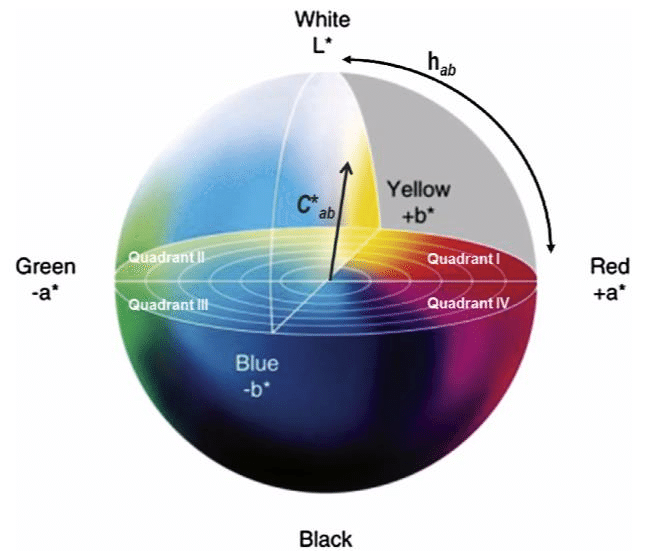
\includegraphics[width=0.8\textwidth]{Lab.png}
    \caption{Visualization of an Lab color representation [TODO ref]} \label{fig:labscheme}
\end{figure}

\chapter{Methodology}\label{chapter:methodology}

TODO chapter introduction/outline

\section{Problem definition}

\begin{enumerate}
    \item The place recognition algorithm receives the data from the unsynchronized sensors, namely the 3D-point cloud from the LiDAR and RGB image from an HD camera. The goal is to recognize if the robot is in the current scene for the first time or if the scene has already been visited. Furthermore, if the scene was already visited, the algorithm must precisely tell which previously visited scene corresponds to the current one. The following steps must be solved:
          \begin{itemize}
              \item Data synchronization
              \item Data fusion
              \item Place recognition
                    \\
              \item \textbf{Input:} 3D Point cloud and RGB image
              \item \textbf{Output:} Id of a corresponding previously visited scene or a new id for the scenes visited for the first time
          \end{itemize}
    \item The place recognition algorithm is integrated with the RatSLAMRos system to solve the SLAM problem.
          \begin{itemize}
              \item \textbf{Input:} 3D Point cloud, RGB image, odometry
              \item \textbf{Output:} estimated robot path
          \end{itemize}
\end{enumerate}
\section{System Architecture}\label{section:systemArchitecture}

This section presents an overview of the architecture of the whole system. The system is decomposed into several Nodes. Together with the  RatSLAM ROS and simulator, the system uses three custom nodes: Data fusion, LV Builder, and LV matching. Furthermore, the system contains two additional nodes that do not influence the algorithm's run but are used for the performance analyses and other help utilities, helping with the development process. The system architecture is presented in Figure \ref{fig:systemArchitecture}. The visualization and topics used only for visualization purposes are omitted for clarity.

\begin{figure}[htpb]
    \centering
    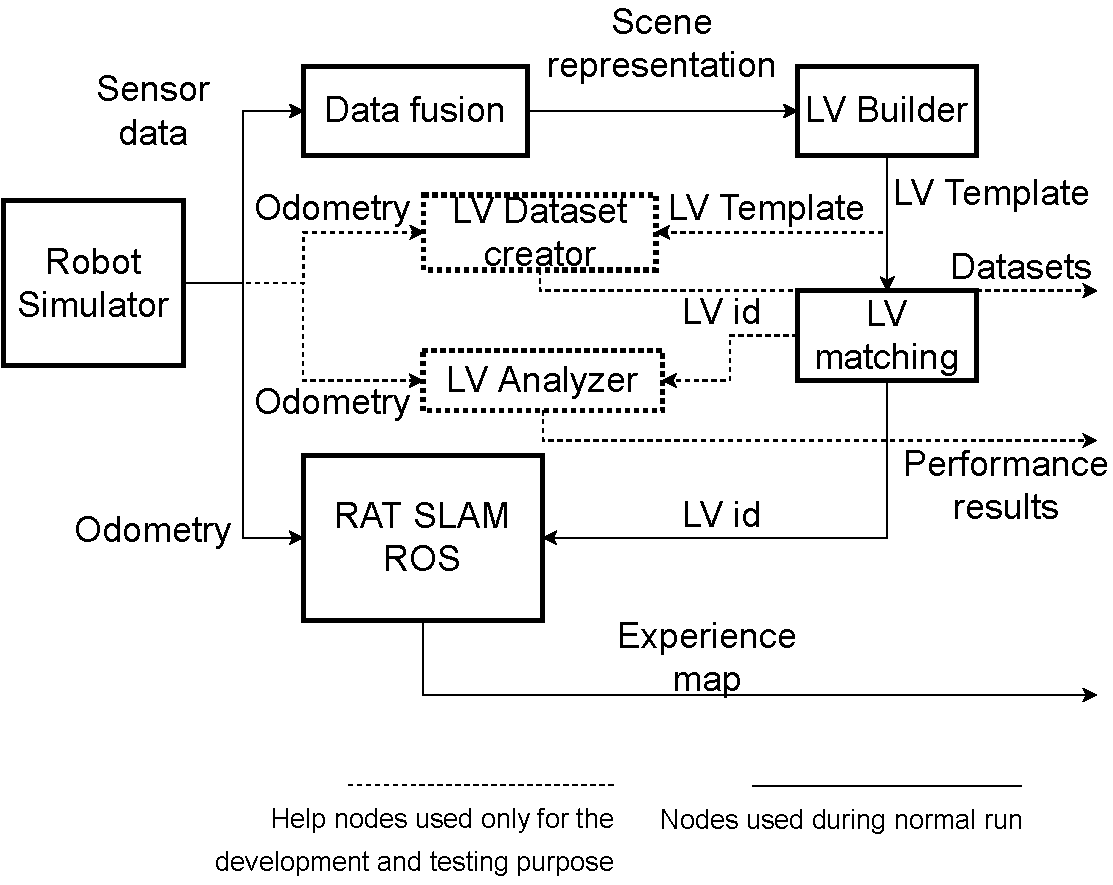
\includegraphics[width=0.8\textwidth]{systemArchitecture.pdf}
    \caption{Diagram of the ROS nodes in the whole system} \label{fig:systemArchitecture}
\end{figure}

\subsection{Robot Simulator}

This node represents the whole simulation and can be easily replaced with a physical robot. The robot is simulated using a Gazebo simulator, introduced in section \ref{section:gazebo}. Besides much other information about the scene and the robot, the simulation publishes data from sensors, namely HD Camera and 3D LiDAR, and odometry data, further consumed by other nodes.

\begin{table}[htpb]
    \caption{Relevant topics published by the simulator}\label{tab:robotSimulatorTopics}
    \centering
    \begin{tabular}{l l l}
        \toprule
        Topic                   & Type                          & Mode    \\
        \midrule
        camera/rgb/camera\_info & sensor\_msgs::CameraInfo      & publish \\
        camera/rgb/image\_raw   & sensor\_msgs::CompressedImage & publish \\
        velodyne\_points        & sensor\_msgs::PointCloud2     & publish \\
        odom                    & nav\_msgs::Odometry           & publish \\
        \bottomrule
    \end{tabular}
\end{table}

\subsection{Data Fusion}

The goal of this node is to take raw data from the sensors and create a single representation of the environment, combining the advantages of each sensor. This node takes care of the synchronization of the sensors, dealing with different frames of reference and the fusion itself. The data fusion node subscribes to the camera and LiDAR topics published by simulation or a real robot and publishes one topic with the final environment representation. How this node exactly works is described in the section \ref{section:fusion}.

\begin{table}[htpb]
    \caption{Subscribed and published topics by the Data fusion node}\label{tab:dataFusionTopics}
    \centering
    \begin{tabular}{l l l}
        \toprule
        Topic                   & Type                          & Mode      \\
        \midrule
        camera/rgb/camera\_info & sensor\_msgs::CameraInfo      & subscribe \\
        camera/rgb/image\_raw   & sensor\_msgs::CompressedImage & subscribe \\
        velodyne\_points        & sensor\_msgs::PointCloud2     & subscribe \\
        rgb\_cloud              & sensor\_msgs::PointCloud2     & publish   \\
        \bottomrule
    \end{tabular}
\end{table}

\subsection{LV Builder}

This node subscribes single topic published by the Data Fusion node. The main task of this node is to take the environment representation and reformat it into a suitable template that will be stored in a memory and compared with previously visited scenes. This node publishes a topic with the built template and two other topics for visualization and debugging purposes. Different approaches to the exact implementation of this node are described in the sections \ref{section:placeOutline} - \ref{section:2stage}.

\begin{table}[htpb]
    \caption{Subscribed and published topics by the LV Builder node}\label{tab:lvBuilderTopics}
    \centering
    \begin{tabular}{l l l}
        \toprule
        Topic                      & Type                                                    & Mode      \\
        \midrule
        rgb\_cloud                 & sensor\_msgs::PointCloud2                               & subscribe \\
        current\_scene\_descripion & msgs::LVDescription\tablefootnote{Self defined message} & publish   \\
        clustered\_viz             & sensor\_msgs::PointCloud2                               & publish   \\
        convex\_hull\_viz          & sensor\_msgs::PointCloud2                               & publish   \\
        \bottomrule
    \end{tabular}
\end{table}
\subsection{LV Matching}

This node subscribes to a topic published by the LV Builder node. The goal of this node is to store all visited places, assign unique ids to all seen scenes, compare a received scene with other scenes, and decide if it was already seen. If the currently received scene template is similar enough to some of the stored templates, this node publishes the id of the matched template. If there is no such template, this node generates and publishes a brand new id and stores the received template as a newly visited place. The only topic this node is publishing is a topic with ids of matched or new scenes.

\begin{table}[htpb]
    \caption{Subscribed and published topics by the LV Matching node}\label{tab:lvMatchingTopics}
    \centering
    \begin{tabular}{l l l}
        \toprule
        Topic                      & Type                       & Mode      \\
        \midrule
        current\_scene\_descripion & msgs::LVDescription        & subscribe \\
        LocalView/Template         & ratslam\_ros::ViewTemplate & publish   \\
        \bottomrule
    \end{tabular}
\end{table}

\subsection{Rat SLAM ROS}

This diagram block represents not a single node but a whole package from several nodes. This is an OpenRatSLAM described in section \ref{section:ratSlamRW}, run without almost any changes. The only difference compared to the original package is the number of started nodes. The lv Node is not activated because its job is done by LV Builder and LV Matching node, and the visual odometry Node is replaced by an odometry sensor from the simulator. The package subscribes to the topic with scene ids published by the LV matching node and to the topic with odometry directly from the simulator. The only relevant published topic is the experience map topic, with the final experience map, which is the final result of the whole algorithm.

\begin{table}[htpb]
    \caption{Relevant subscribed and published topics by the RatSLAMRos package}\label{tab:ratslamTopics}
    \centering
    \begin{tabular}{l l l}
        \toprule
        Topic              & Type                         & Mode      \\
        \midrule
        LocalView/Template & ratslam\_ros::ViewTemplate   & subscribe \\
        odom               & nav\_msgs::Odometry          & subscribe \\
        ExperienceMap/Map  & ratslam\_ros::TopologicalMap & publish   \\
        \bottomrule
    \end{tabular}
\end{table}

\subsection{LV Analyzer}

This node subscribes to the same topics as the Rat SLAM ROS package. This node serves only debugging purposes and does not influence the algorithm. The goal of this node is to evaluate the performance of the algorithm. It receives all the ids of matched scenes and new ids from the LV Matching node and can pair them with the exact position of the robot at the time the scene template was taken because of the information received from the simulator. This node remembers the precise position of each scene newly remembered by the LV Matching node and can calculate the position difference between each match and the original matched scene. Furthermore, it can calculate the distance to the nearest previously visited scene for each newly added template. According to the metrics described in the section \ref{section:Evaluation}, the number of false positive and false negative matches can be calculated, leading to the approach's final accuracy, recall, and precision. These estimated numbers are the final output of this node.


\begin{table}[htpb]
    \caption{Subscribed  topics by the LV Analyzer node}\label{tab:lvAnalTopics}
    \centering
    \begin{tabular}{l l l}
        \toprule
        Topic                 & Type                          & Mode      \\
        \midrule
        LocalView/Template    & ratslam\_ros::ViewTemplate    & subscribe \\
        odom                  & nav\_msgs::Odometry           & subscribe \\
        camera/rgb/image\_raw & sensor\_msgs::CompressedImage & subscribe \\
        \bottomrule
    \end{tabular}
\end{table}

\subsection{LV Dataset Creator}\label{section:lvdatasetCreator}

This node works in principle similarly to the LV Analyzer node. The goal of this node is to pair the templates with their exact positions received from the simulator. Unlike the LV Analyzer node, this node receives and pairs the whole template from the LV Builder node instead of only the scene id from the LV Matching node. The set of pairs of templates and their exact positions is the output of this node, which helps build final datasets for automatic parameter tuning, see section \ref{section:parameterTuning}, or neural networks training, see section \ref{section:nnTraining}.


\begin{table}[htpb]
    \caption{Subscribed  topics by the Dataset creator node}\label{tab:datasetCreatorTopics}
    \centering
    \begin{tabular}{l l l}
        \toprule
        Topic                      & Type                & Mode      \\
        \midrule
        current\_scene\_descripion & msgs::LVDescription & subscribe \\
        odom                       & nav\_msgs::Odometry & subscribe \\
        \bottomrule
    \end{tabular}
\end{table}
\section{Data fusion and preprocessing}

This section introduces the process of processing the raw data received from the sensors and creating a final representation of the environment that is further used as an input for the other stages of the process.\par
In this thesis, we receive colored 2-dimensional images from an HD camera and a raw 3D point cloud from a 3D lidar sensor. The goal is to use these two inputs and generate a colored point cloud for a more accurate environment representation.\par
In this work, we assume that both sensors are calibrated and that the excentric parameters, namely field of view and transformation matrix between sensor's frames, are already known. If this is not the case, some of the following well-known techniques (TODO ref) can be used for their determination.\par
The whole process can be divided into three major parts. In the beginning, the frequencies of the sensors must be synchronized. Then, after the input data are synchronized, the data fusion is performed, and the individual scene representations are merged into one mutual model, containing information from all individual sensors. Finally, the built representation is preprocessed and simplified by removing the unnecessary data, especially the information about the ground. The whole process is visualized in Figure \ref{fig:dataFusionWorkflow} and each step is described in the following subsections.

\begin{figure}[htpb]
    \centering
    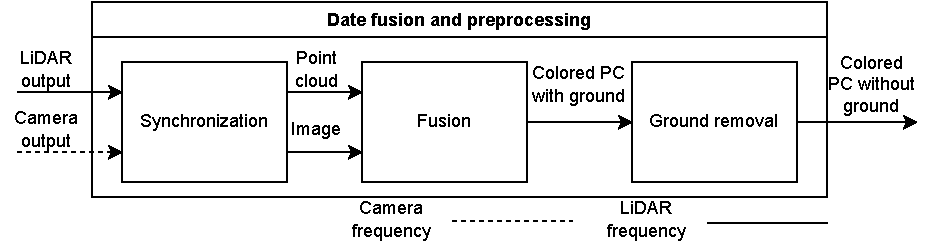
\includegraphics[width=0.8\textwidth]{dataFusionWorkflow.pdf}
    \caption{Caption} \label{fig:dataFusionWorkflow}
\end{figure}

Figure \ref{fig:dataFusionExample} illustrates example inputs received from the sensors (a) and (b), generated output after the data fusion (c), and final generated output after the ground removal (d).

\begin{figure}[!tbp]
    \centering
    \subfloat[Input received from the camera.]{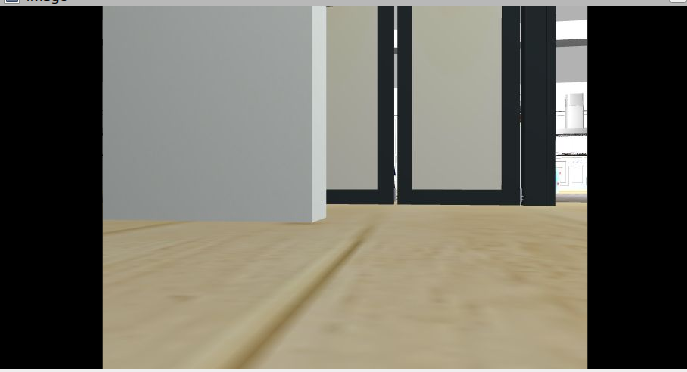
\includegraphics[height=0.2\textheight]{dataFusionExampleImage.png}\label{fig:dataFusionExample1}}
    \hfill
    \subfloat[Input received from the LiDAR.]{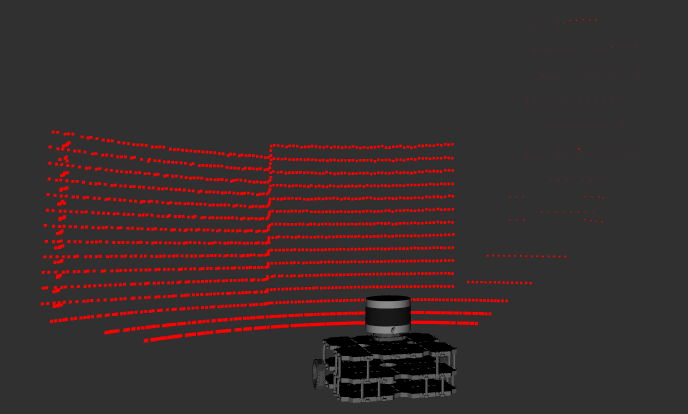
\includegraphics[height=0.2\textheight]{dataFusionExampleRawCloud.png}\label{fig:dataFusionExample2}}
    \\
    \subfloat[Colored point cloud after data fusion]{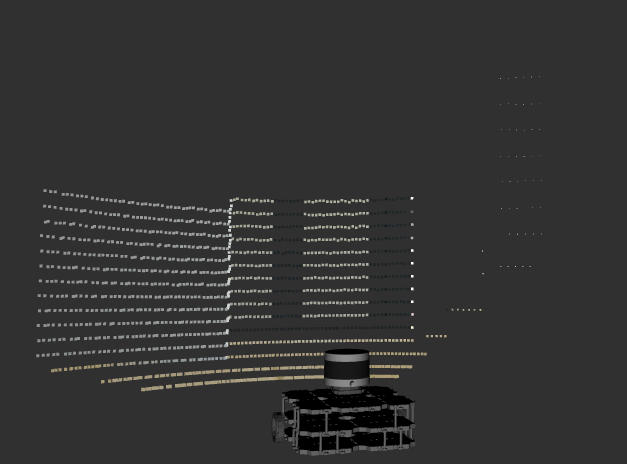
\includegraphics[height=0.2\textheight]{dataFusionExampleColoredCloud.png}\label{fig:dataFusionExample3}}
    \hfill
    \subfloat[Final result after the ground removal]{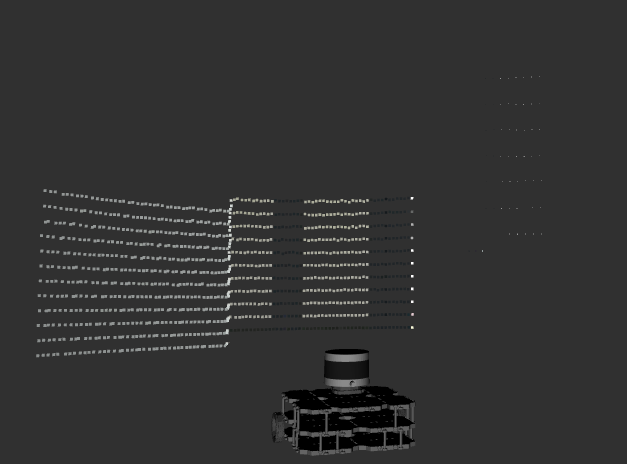
\includegraphics[height=0.2\textheight]{dataFusionExampleFinal.png}\label{fig:dataFusionExample4}}
    \caption{Data fusion sensors inputs and generated outputs after each stage}
    \label{fig:dataFusionExample}
\end{figure}

\subsection{Sensors synchronization}

This section solves the problem that the sensors deliver data at different times with different frequencies. The goal of the synchronization is to receive unsynchronized data from both sensors and return synchronized pairs of images and point clouds that will be used for further fusion.\par
The technique used in this thesis is based on the assumption that the camera frequency is significantly larger than the frequency of the 3D-lidar\footnote{In the experiments, we used a camera that has 15 times higher frequency than the 3D-lidar.}. Based on this fact, the system can just record all the images received from the camera. All point clouds received from the 3D-lidar are afterward paired with the last received image.\par
The time difference between the image and point cloud is so low, compared to the frequency of the lidar, that it can be neglected, and we can assume that the image and the point cloud were taken simultaneously.

\subsection{Data fusion}

At this point, we assume that all the data are synchronized and working with a pair of images and raw point clouds representing the same scene at the same time. (TODO also assumes the same frame?). The goal is to build a colored 3D point cloud.\par
The point cloud $PC$ is represented as an unordered set of triples, describing a single point's $x, y, z$ coordinates:
$$
    PC \subseteq \left\{ (x,y,z) | (x,y,z) \in \mathbb{R}^3\right\}.
$$
The image can be represented as a function $img: \mathbb{R}^2 \rightarrow \mathbb{N}_0^3 \cup \{0\}$ taking $x,y$ pixel coordinates as input and returning RGB representation of the pixels color or 0, if the give coordinates are out of range\footnote{If $x$ or $y$ are not the whole numbers, they are rounded to the nearest whole number.}:
$$
    img(x,y) = \begin{cases}
        (r,g,b) & \text{if $(x,y)$ are inside of the cameras field of view} \\
        0       & \text{otherwise,}
    \end{cases}
$$
where $r,g,b$ corresponds to the pixel color's red, green, and blue parts.\par
The result $CPC$ will be represented as an unordered set of sextuplets, describing a single point's $x, y, z$ coordinates together with $r, g, b$ colors:
$$
    CPC \subseteq \left\{ (x,y,z,r,g,b) | (x,y,z,r,g,b) \in \mathbb{R}^3 \times \mathbb{N}_0^3 \right\}.
$$\par
Let $\mathbf{P}$ be the projection matrix that projects 3D world coordinates into the 2D pixel coordinates on the image plane using the following formula:
$$
    \mathbf{x} = \mathbf{P}\mathbf{X},
$$
where $\mathbf{X} = \left[x_\text{world},y_\text{world},z_\text{world}\right]^T$ represents a 3D world coordinates vector and $\mathbf{x} = \left[x_\text{image}, y_\text{image}\right]^T$ represents a 2D image plane coordinates vector. This matrix can be found using the camera's and lidar's excentric parameters received from the calibration [TODO ref].\par
If we know the projection matrix $\mathbf{P}$, we can iterate through all the points in the point cloud, project them into the image plane, find the corresponding pixel and bind its color with the examined point. All points outside the camera's field of view shall be ignored and not included in the result.\par
The algorithm for the fusion of the data received from Lidar and camera is summarized in the Algorithm \ref{alg:fusion}.

\begin{algorithm}
    \caption{Lidar and camera data fustion}\label{alg:fusion}
    \begin{algorithmic}
        \Require Point cloud $PC$, camera image $img$
        \Ensure Colored point cloud $CPC$
        \State $CPC := \{\}$  \Comment{Initialize result as an empty set}
        \State $\mathbf{P} \leftarrow $ build projection matrix
        \For{$(x,y,z) \in PC$} \Comment{Iterate through all points in $PC$}
        \State $[x_i,y_i]^T \leftarrow  \mathbf{P}\cdot[x,y,z]^T$ \Comment{Project current point to the image plane}
        \If{$img(x_i,y_i) \neq 0$} \Comment{Ignore points out of cameras field of view}
        \State $(r,g,b) \leftarrow  img(x_i,y_i)$  \Comment{Get projected pixel color}
        \State $CPC \leftarrow CPC \cup \{(x,y,z,r,g,b)\}$  \Comment{Add colored point to the result}
        \EndIf
        \EndFor
        \State\Return $CPC$
    \end{algorithmic}
\end{algorithm}

\subsection{Ground removal}

Ground removal is a widely used technique, applied by many algorithms working with 3D clouds. Even if the information about the ground, particularly about the ground color, might help distinguish between two different scenes, the points representing the floor are usually in the same position for every scene and therefore carry a relatively small information value. Removing these points can significantly reduce the input size, with minimal loss of the information value, which can positively influence the algorithm's performance. Furthermore, the ground points may connect two completely separate objects and therefore have a negative influence on the scene segmentation or object detection algorithms.\par
Let's assume that all points from the points cloud are represented in the world's frame of reference and that $y$ ax is orthogonal to the ground. Then, it is evident that there exists a threshold $y_{th}$, such that all points representing a ground have $y$ coordinate lower or equal to the $y_{th}$ and all other points will have $y$ coordinate larger than $y_{th}$. So, if the threshold $y_{th}$ is known\footnote{This threshold can be very easily determined experimentally.}, the ground point can be removed simply by filtering the points by their $y$ coordinate. The ground removal process is summarized in the Algorithm \ref{alg:groundRemoval}.

\begin{algorithm}
    \caption{Ground removal}\label{alg:groundRemoval}
    \begin{algorithmic}
        \Require Colored point cloud $CPC$, threshold $y_{th}$
        \Ensure Colored point cloud $CPC_2$ without ground
        \State $CPC_2 := \{\}$  \Comment{Initialize result as an empty set}
        \For{$(x,y,z,r,g,b) \in CPC$} \Comment{Iterate through all points in $CPC$}
        \If{$y > y_{th}$} \Comment{Ignore points under the threshold}
        \State $CPC_2 \leftarrow CPC_2 \cup \{(x,y,z,r,g,b)\}$  \Comment{Add current point to the result}
        \EndIf
        \EndFor
        \State\Return $CPC_2$
    \end{algorithmic}
\end{algorithm}

Besides the ground, this method can remove some other objects' bottom parts, like the feet of pedestrians, wheels of wheelchairs, etc., which can lead to a slightly more significant information loss than pure ground removal. However, there exist other, better ground removal techniques, usually based on machine learning, which do not suffer from this issue [TODO refs]. Yet, these techniques typically require more computational resources than the simple filtering approach, and the results are usually not significantly different\footnote{Especially in the indoor environments with static objects like furniture, which are in the main focus of this work}, so we decided to prefer this simple method despite the minor quality drawbacks.
\section{General place recognition outline}\label{section:placeOutline}

After the data are fused into a uniform scene representation, the place recognition is performed. This algorithm aims to remember all places the robot has visited and to decide if the current scene, received from the sensors, has been already visited or not, and eventually return the unique identification of the previously visited place.\par
In order to achieve this goal, we need to find a suitable representation (further template) of the place that will be remembered by the robot. This template must be created from the fused scene description received from the sensors, should occupy little space, and be easy to compare.\par
The place recognition algorithm works in three steps. In the first step, the designed template is built from the received fused scene representation. In the second step, this template is independently compared with all the stored templates, representing previously visited places. A template comparison result is a real number between 0 and 1, representing the similarity of both templates. The closer the similarity to 1, the more similar the templates are. After all the templates are compared, the most similar template is chosen. In the last step, the similarity of the most similar template is compared to the given threshold. If it is greater, the most similar template is returned as the same place. If it is smaller, the current template will be remembered, and the result will be that this place was not visited before. The whole process is visualized in Figure \ref{fig:placeRecognitionWorkflow}.\par

\begin{figure}[htpb]
    \centering
    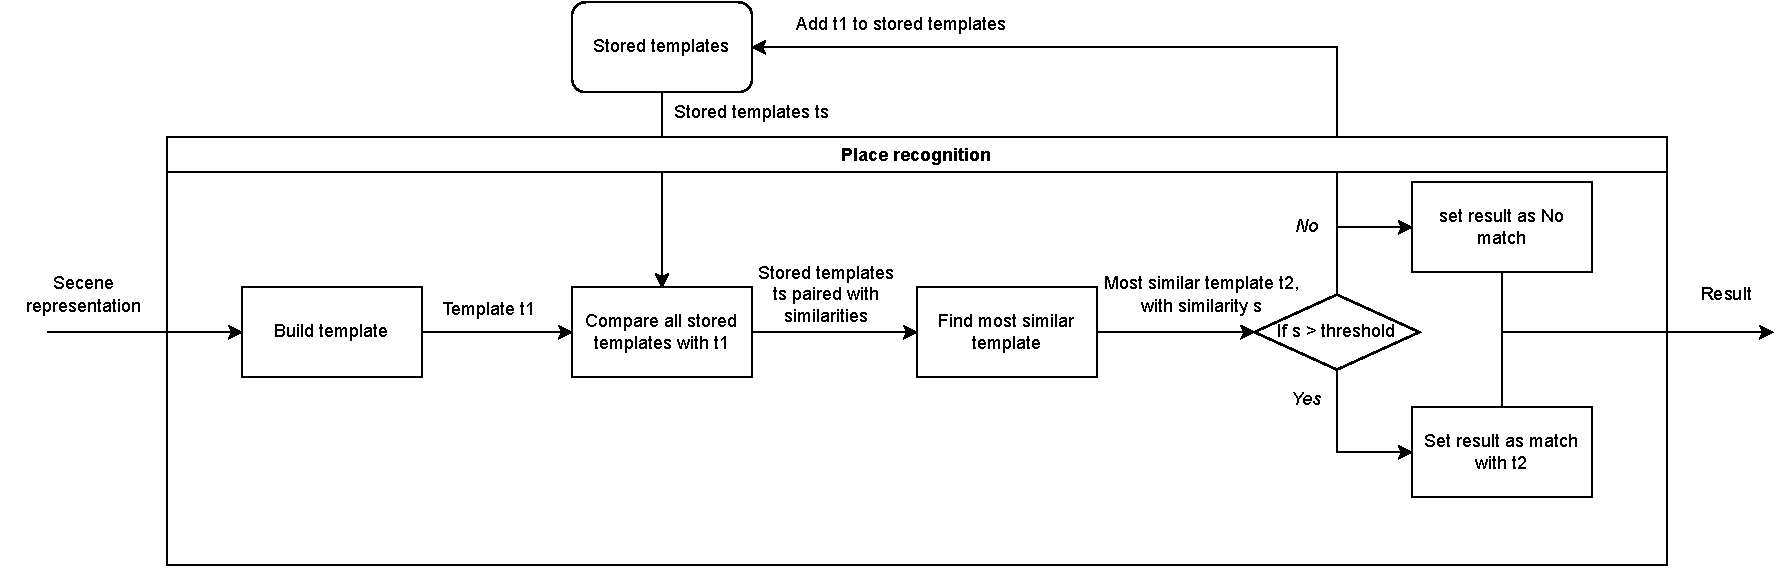
\includegraphics[width=0.8\textwidth]{placeRecognitionWorkflow.pdf}
    \caption{Common place recognition workflow} \label{fig:placeRecognitionWorkflow}
\end{figure}

The following sections suggest three different approaches to place recognition. All presented techniques differ in template structures and template building and comparison algorithms. Otherwise, they all share the same structure shown in this section.
\section{Hierarchical view matching based on Clustering}\label{section:hierarchical}

The first place recognition method presented in this work found inspiration in the human memory of places. Unlike the further proposed methods, this approach does not try to model the brain's other biological structures but tries to conceive biological inspiration more abstractly. The idea is based on the way how humans usually remember places. According to the [TODO refs], the long-term human spatial memory recall is built upon a hierarchical structure. First, people remember the general layout of the view. Afterward, they can recall basic information about the scene's largest or most significant features, followed by a few more detailed features. Finally, the small details are usually wholly forgotten or recalled at last.\par
The template representation is used based on this behavior. The scene is decomposed into a set of objects based on their location, connection, and color. Each object is simplified as a list of its most significant features, namely the position of its center point, volume and area of its convex hull, and its most significant color. Together with this information, the number of points from the colored point cloud in this object is stored. Afterward, the small, insignificant objects are entirely ignored.\par
During the matching process, the scenes are compared according to these objects. Objects are paired by their similarities based on their stored properties' similarities. The final similarity is calculated as a weighted average of these similarities by the number of points connected with the object. In this way, the largest, usually most significant objects influence the result more than the smaller details.\par

TODO images of an example - scene/representation

\subsection{Template extraction}

The decomposition of the colored point cloud into the set of objects description is a two-step process. In the first step, the scene is decomposed into clusters, representing individual objects. Afterward, in the second step, all clusters are processed independently, and the objects' information is extracted.\par
The clustering is performed using the DBScan algorithm [TODO reference] in a six-dimensional space. The first three dimensions standardly represent the points' x, y, and z positions. The additional three dimensions represent points' colors, namely the red, green, and blue components. The standard DBScan algorithm assumes that all dimensions are in the same units. Because there is obviously no standard conversion between color and distance, the color dimensions must be scaled by a suitable scaling factor. The best coefficient has been found experimentally, as well as the DBScan parameters.\par

TODO image of scene before and after the clustering

After the scene is decomposed, each cluster is processed independently of the others. Before the information about the object is extracted,  its convex hull is found using the quick-hull algorithm [TODO ref]. After the convex hull is known, its center, volume, and area can be easily calculated. [TODO reference] Together with the information obtained from the convex hull, the information about the object's color is extracted. Based on the properties of the DBScan algorithm, it can be expected that all points from the cluster have a similar color. Therefore, storing average color instead of all individual colors leads to negligible information loss. The average color is calculated as an arithmetic average of the red, green, and blue parts of the colors of individual points in the cluster. After calculating, the average color is converted into the chosen color format. [TODO chapter reference] The last stored information about the object is the cluster size\footnote{Number of points in the cluster}.\par
All clusters with a size smaller than the given threshold are considered small insignificant objects and are ignored even before the object information extraction process starts.

TODO diagram of the whole process

\subsection{Template matching}

Before calculating the similarity between two whole scenes, we need to describe an approach for comparison of two objects based only on the object properties. We compare four essential properties of the objects: distance between objects, the difference between colors, sizes, and shapes of the objects. The distance of the objects is calculated as the euclidean distance of their centers. The formulas described in chapter [TODO chapter ref] are used for the color differences. The size difference is calculated as a difference between the volume of the convex hulls of the objects. For the determination and comparison of the exact shapes, we do not have enough information. However, much information about the shape of many objects is encoded in a ratio between their volume and area. There are, of course, objects with entirely different ratios between volume and area, but for most pairs with different shapes, the ratio between volume and area is also different. So the difference between shapes is represented as a difference in the ratio of volume and area of the convex hulls of the objects.\par
At this point, the absolute difference between objects is known for each essential property, and we have to decide if they are similar enough or not. Therefore the function is needed for each property that takes the property difference as an input and returns a number between 0 and 1, representing the similarity of the individual property. In this work, we choose
$$
    f_{a,x_0}(x) = 1 - \frac{1}{1 + e^{-a(x-x_0)}}
$$
as the wanted function for each property, where $x$ is the input, and $a$ and $x_0$ are parameters specific for each property. This function, illustrated in Figure \ref{fig:sigmoid}, has a property that for differences smaller than the threshold, it is very close to one, for differences larger than the threshold, it is close to 0, and for inputs in the neighborhood of the threshold, it is gradually decreasing. The way how to find the suitable parameters is described in the following section.\par

\begin{figure}[htpb]
    \centering
    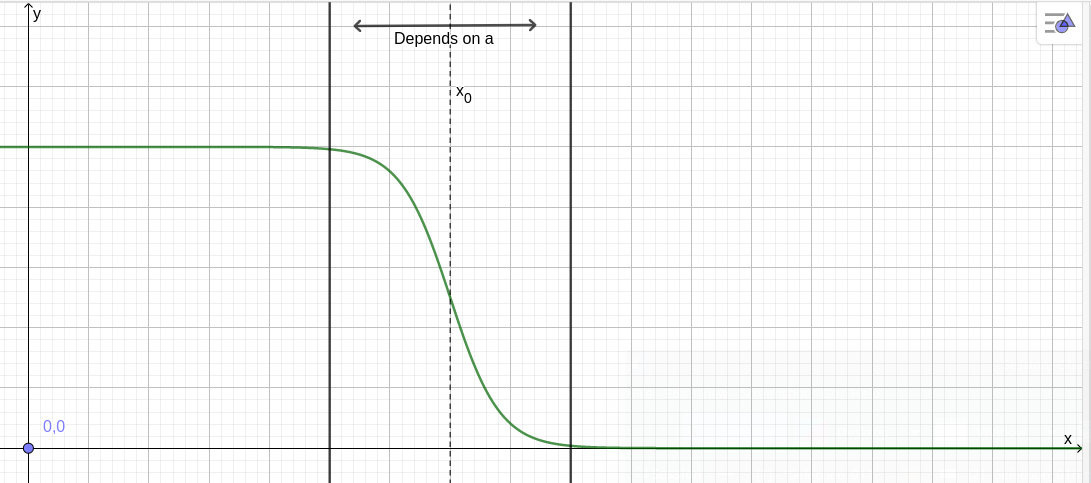
\includegraphics[width=0.8\textwidth]{sigmoid.png}
    \caption{Parametrized sigmoid function} \label{fig:sigmoid}
\end{figure}

After the similarity of each property is calculated, the final similarity of the objects is calculated as a weighted average of the similarities of the individual properties. The weights are found automatically, as described in the following section. The object matching process is summarized in Algorithm \ref{alg:objectSimilarityCalc}.

\begin{algorithm}
    \caption{Objects comparsion}\label{alg:objectSimilarityCalc}
    \begin{algorithmic}
        \Require Objects $O_1$ and $O_2$
        \Ensure Similarity of the objets
        \State $x_1 \leftarrow $ difference in colors between $O_1$ and $O_2$
        \State $x_2 \leftarrow $ difference in positions between $O_1$ and $O_2$
        \State $x_3 \leftarrow $ difference in volume between $O_1$ and $O_2$
        \State $x_4 \leftarrow $ difference in volume/area ration between $O_1$ and $O_2$
        \State $s_1 \leftarrow f_{a_1,x_{0,1}}(x_1)$
        \State $s_2 \leftarrow f_{a_2,x_{0,2}}(x_2)$
        \State $s_3 \leftarrow f_{a_3,x_{0,3}}(x_3)$
        \State $s_4 \leftarrow f_{a_4,x_{0,4}}(x_4)$
        \State $res \leftarrow\frac{w_1s_1 + w_2s_2 + w_3s_3 + w_4s_4}{w_1+w_2+w_3+w_4}$
        \State\Return $res$
    \end{algorithmic}
\end{algorithm}

The method for comparison of the two scenes uses the above-described approach for comparison of the individual objects. First, let's define a scene as an unordered set of objects. Then, let's define the primary scene as the current scene received from the sensors and the secondary scene as the scene from the storage. This approach iterates through all objects in the primary scene and, for each object, calculates the similarities with all objects in the secondary scene. Afterward, for each object in the primary scene, the most similar object from the secondary scene is picked\footnote{Two objects in the primary scene may have the same most similar object from the secondary scene}. Finally, the similarities with the most similar objects are used to calculate the average, weighted by the sizes of the clusters. The whole process is summarized in the Algorithm \ref{alg:scenesSimilarityCalc}.

\begin{algorithm}
    \caption{Scenes comparsion}\label{alg:scenesSimilarityCalc}
    \begin{algorithmic}
        \Require Primary scene $S_1$ and secondary scene $S_2$
        \Ensure Similarity of the scenes
        \State $res := 0$
        \State $sizesTotal := 0$
        \For{$o_1 \in S_1$}
        \State $best := 0$
        \For{$o_2 \in S_2$}
        \State $best \leftarrow \max(best,\text{ CompareObjects($o_1,o_2$)})$
        \EndFor
        \State $res \leftarrow left + best \cdot \text{clusterSize($o_1$)}$
        \State $sizesTotal \leftarrow sizesTotal + \text{clusterSize($o_1$)}$
        \EndFor
        \State $res \leftarrow \frac{res}{sizesTotal}$
        \State\Return $res$
    \end{algorithmic}
\end{algorithm}

\subsection{Automatic parameter tuning}\label{section:parameterTuning}

To make the templates comparison algorithm work, 13 different parameters must be correctly set. Namely, $a$ and $x_0$ parameters for the sigmoid functions for each of four property differences, the weight of each property, and the final threshold. There are naturally many combinations, and every change may strongly influence the results and the optimal values of the other parameters, so manual setting of these parameters wouldn't bring satisfactory results. Therefore, an automatic optimization method that minimizes the number of errors based on the choice of the correct parameters is required.\par
In this work, we used genetic algorithms. [TODO reference] The minimized fitness function is a count of false positive and false negative evaluations after a simulation of a robot run in a prepared environment. The simulation, environments, and evaluation metrics are the same as those used for the performance testing and are described in chapters [TODO chapters reference]. In some cases, like usage of the approach for the 2-Stage matching, see chapter [TODO chapter reference], it might be beneficial to minimize the number of false positives at the expanse of false negatives or vice versa. In this case, we can appropriately weigh the number of false positives and negatives in the final sum.
\section{Neural Networks based view matching}

The second technique offered in this work is based on neural networks. This approach is not designed as a standalone method but is presented only as a proof of concept and further used in the 2-Stage approach presented in the chapter [TODO chapter reference]. The used neural network is inspired by siamese neural networks [TODO ref].\par
These networks usually consist of two parts and are typically designed to compare any two entities. The first part consists of two networks with the same structure and usually with shared weights. This part is used for the automatic feature extraction from the input entities. The second part consists of a single network taking feature vectors extracted by both neural networks in the first part, performing the desired operation on the entities, and building corresponding output. In the case of comparison network is the output of the second part, and therefore of the whole network, a single number between 0 and 1, determining the similarity of the entities. The typical structure of a siamese neural network is shown in Figure \ref{fig:siamseNetwork}.

\begin{figure}[htpb]
    \centering
    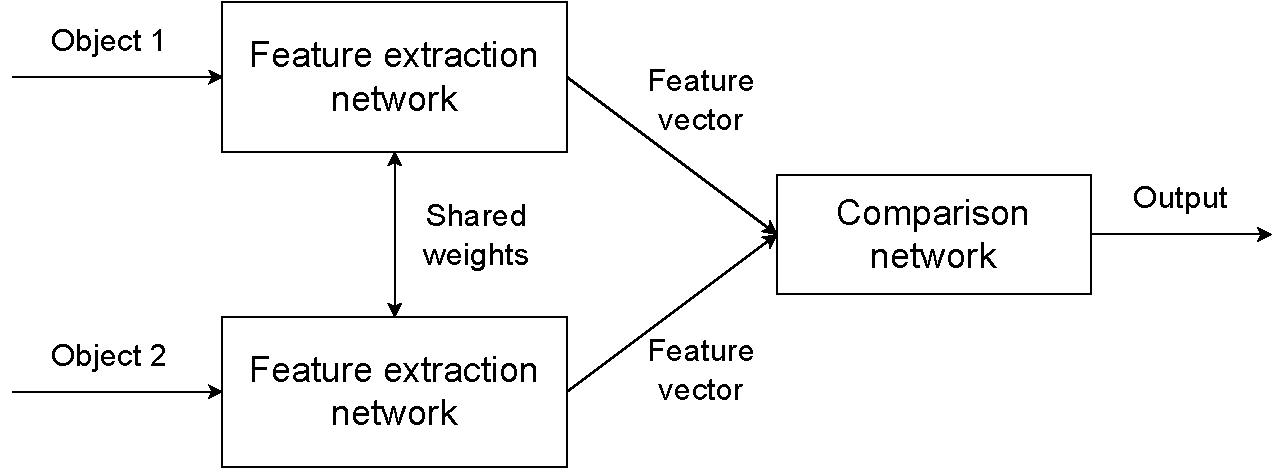
\includegraphics[width=0.8\textwidth]{siamseNetwork.pdf}
    \caption{Example of a siamese network used for object comparison} \label{fig:siamseNetwork}
\end{figure}

\subsection{Networks structure}

In this work, a slightly modified PointNet network, see chapter [TODO chapter ref], is used as a feature extractor. The only modification compared to the original networks is in the sizes of the layers and the output because we are typically working with significantly more sparse point clouds than the network designers\footnote{The exact parameters of the network are stated in the attachments [TODO add params to the attachment]}. As a result, the extracted feature vector contains only 256 numbers instead of 1024.\par
The feature vector extracted by this network is the scene template extracted from each input, processed in the future steps, and eventually stored in the storage.\par
The two extracted feature vectors are further compared by a single multilayer perceptron network (further MLP). This network has 512 input neurons and produces a single output. The network takes as input a concatenation of both feature vectors and produces a number between 0 and 1, describing the similarity of the scenes represented by given feature vectors. Several architectures of the networks were tried, but the best results were produced by a network with a single hidden layer containing 256 neurons and with a sigmoid as an activation function on the output neuron.

\subsection{Training of the networks}\label{section:nnTraining}

Both networks are trained separately. For the training of the PointNet, used for the feature extraction, we used an original algorithm presented in [TODO reference]. In order to be able to evaluate the results and compare them with the expected results in the dataset, the PointNet network was concatenated with a simple MLP network used for the object classification. Then, the whole classification network was trained on the [TODO dataset link] dataset. After the classification network was trained, the final MLP network was removed, and the first PointNet part was used as a trained model for the feature extraction.\par
The second part of the network, namely the MLP comparing two feature vectors, was trained using a backpropagation algorithm [TODO ref] based on the mean squared error loss function [TODO ref]. The dataset was generated from a sample simulation, see chapter [TODO chapter ref]. During the simulation, the trained feature extractor network creates a feature vector from each scene. Afterward, a set of all pairs of the feature vectors is made. A random subset was chosen from this set, and all couples from this subset were labeled using exact scene locations received from the simulator and the criteria described in the chapter [TODO chapter ref]. This labeled subset was used as a training set for the MLP network.

\section{2-stage View Matching}\label{section:2stage}

This approach tries to combine both previously presented methods to achieve better results. The first approach works pretty well in many scenes but has one drawback. Since the objects' shapes are mainly ignored, taking into account only the ratio between the volume and the area of the objects, there could be many scenes with similarly placed objects with similar sizes but different shapes. This could lead to many unwanted false positive evaluations. This approach tries to use neural networks presented in section \ref{section:nnMatching} to eliminate these false positives while maintaining most of the advantages of the first approach, described in section \ref{section:hierarchical}.\par

\subsection{Template Building}

The scene representation in this method combines the scene representations from both previously presented techniques. The scene is represented as a set of objects description, as described in section \ref{section:hierarchical}, and simultaneously, the feature extraction described in section \ref{section:nnMatching} is performed. The Final representation is a tuple of the object decomposition and features vector.

\subsection{Template Matching}

As the name of the approach suggests, the matching is performed in two stages. In the first stage, the similarity of the two scenes is calculated the same as in the section \ref{section:hierarchical}. After the similarity is computed, it is compared with a given threshold so that it is predecided, if it is positive or negative. The calculated similarity is returned as a final result if it is negative. If it is positive, the second stage is performed in order to reduce the number of false positives.\par
In the second stage, the feature vectors are compared in the same way as in a section \ref{section:nnMatching}. If the result is higher than another threshold, the result of the first stage is returned. If the result is lower than the threshold, 0 is returned. The whole process is summarized in Figure \ref{fig:twoStageDiagram}.

\begin{figure}[htpb]
    \centering
    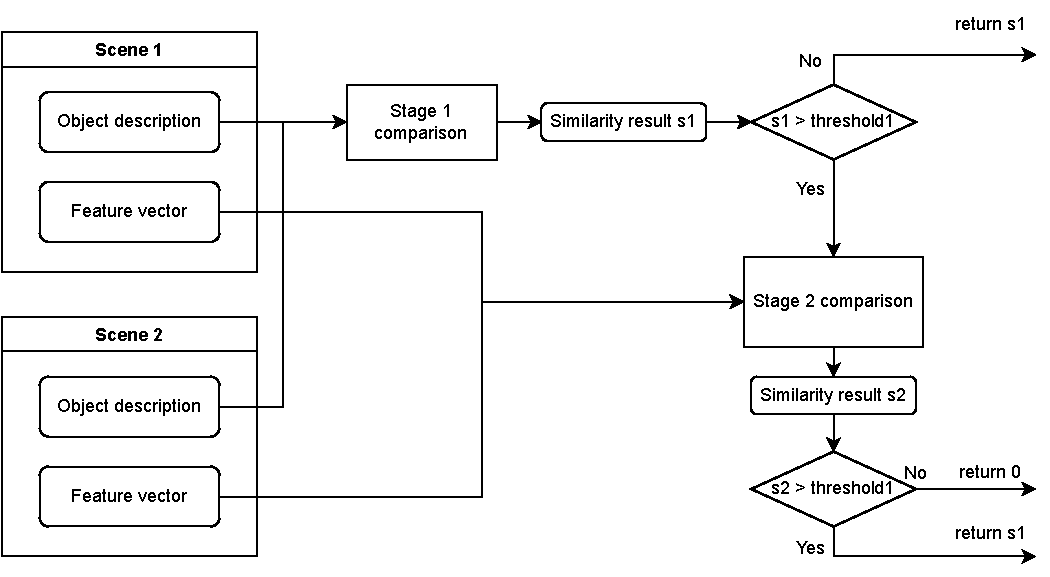
\includegraphics[width=0.8\textwidth]{2stageApproach.pdf}
    \caption{Overview of the two-stage approach} \label{fig:twoStageDiagram}
\end{figure}
\chapter{Experiments}\label{chapter:experiments}

In this section, all presented algorithms will be tested using different metrics and compared with the visual place recognition used in the original RatSLAM approach, described in section \ref{section:ratSlamRW}. The beginning of the chapter will introduce the robot simulator and the environments used for the tests. The following section formally defines the evaluation metrics. The next section will present the system setup of the experiments. In the following four sections, the results of the different evaluation metrics will be discussed. In the penultimate section will be tested the integration of the place recognition approaches with RatSLAM. Finally, the last section will summarize all measured results and discuss the final performance and advantages or disadvantages of all suggested techniques.

\section{Used environments}\label{section:environments}

The system has been tested using a gazebo simulator, described in the section \ref{section:gazebo}. As a robot model, the turtlebot3 waffle PI, described in section \ref{section:turtlebot}, was used and slightly modified with a 3D LiDAR sensor \cite{VelodyneSimulator}. The most important parameters of the robot are summarized in the table \ref{tab:turtlebot}.

\begin{table}[htpb]
    \caption{Turtlebot3 Waffle PI specification}\label{tab:turtlebot}
    \centering
    \begin{tabular}{l l l l l l}
        \toprule
        \textbf{width} & \textbf{height} & \textbf{depth} & \textbf{max speed} & \textbf{cam. frequency} & \textbf{LiDAR frequency} \\
        281 mm         & 141 mm          & 306 mm         & 0.69 ms${}^{-1}$   & 30 Hz                   & 2 Hz                     \\
        \bottomrule
    \end{tabular}
\end{table}

The robot has been tested in three different environments: Warehouse world \cite{WarehouseWorld}, House world \cite{HouseWorld} and Hospital world \cite{HospitalWorld}.\par
The warehouse world, shown in the figure \ref{fig:warehouseWorld}, is a representative environment for most industrial environments in which many robots find an application.\par

\begin{figure}[htpb]
    \centering
    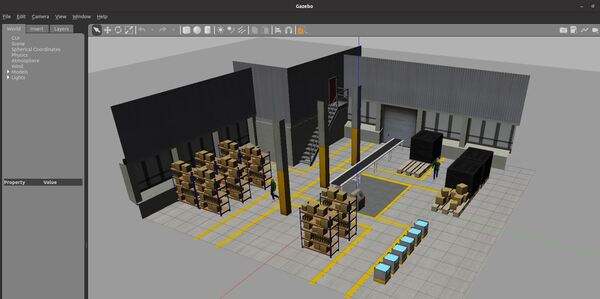
\includegraphics[width=0.8\textwidth]{warehouseEnvironment.jpg}
    \caption{The warehouse world environment [TODO better image]} \label{fig:warehouseWorld}
\end{figure}

The House world, shown in the figure \ref{fig:smallHouse}, represents a typical small, fully equipped apartment. Compared to the warehouse, this environment is significantly smaller and contains more various objects of different shapes and colors. Many of the typical household robots, like robotic vacuum cleaners, will deal with environments like this.\par

\begin{figure}[htpb]
    \centering
    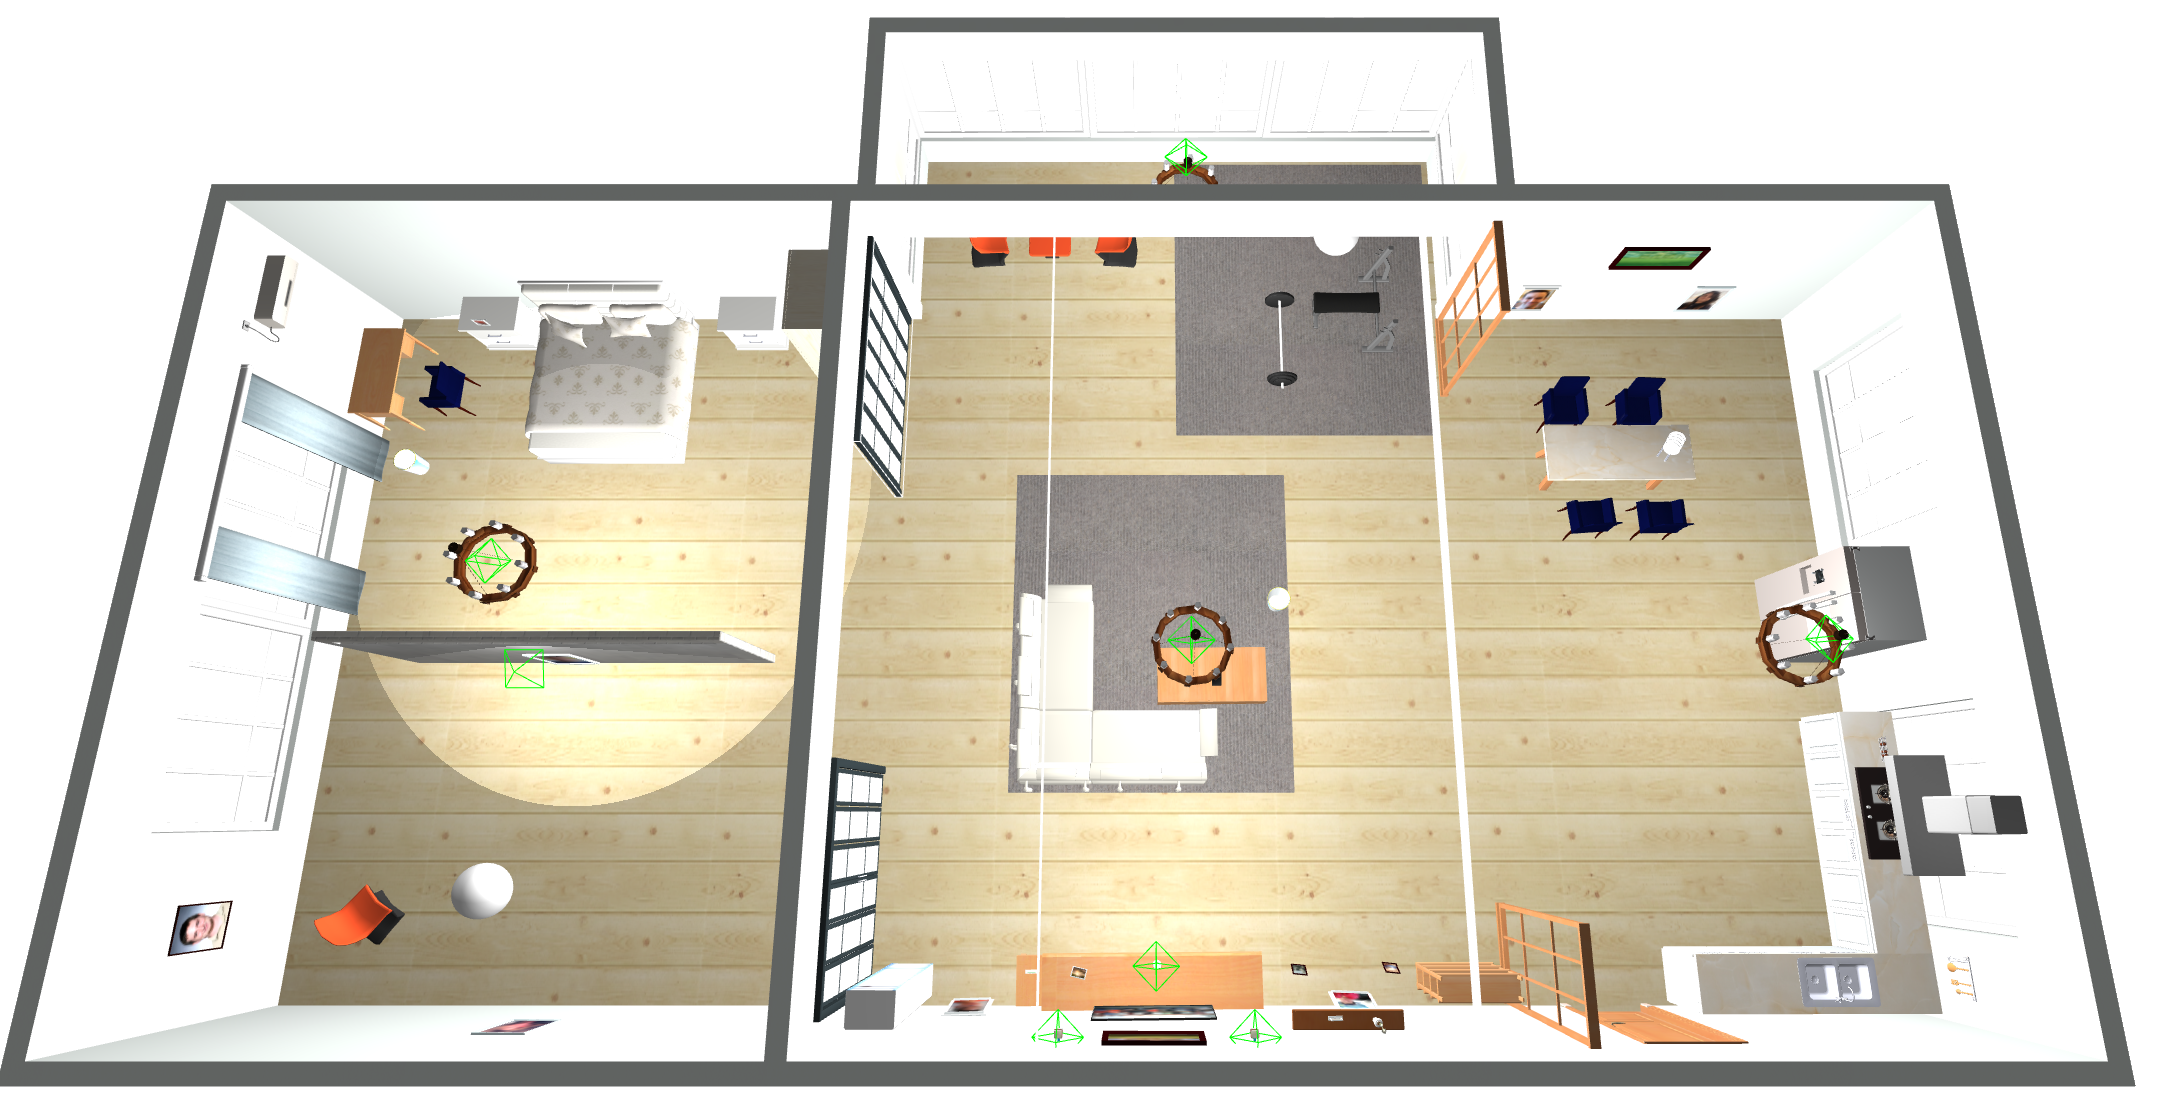
\includegraphics[width=0.8\textwidth]{smallHouse.png}
    \caption{The small house world environment [TODO ref]} \label{fig:smallHouse}
    % https://github.com/aws-robotics/aws-robomaker-small-house-world/blob/ros1/docs/images/gzweb_aws_house.png
\end{figure}

Finally, the hospital world, shown in the figure \ref{fig:hospitalWorld}, is a large, mostly empty environment from the hospital building. This environment is mostly symmetric and contains many places that look very similar, even if they are at opposite building sites. This environment was included mainly to test the algorithm's robustness against these symmetric places. Furthermore, this environment is a typical representation of any office or similar public building.\par

\begin{figure}[htpb]
    \centering
    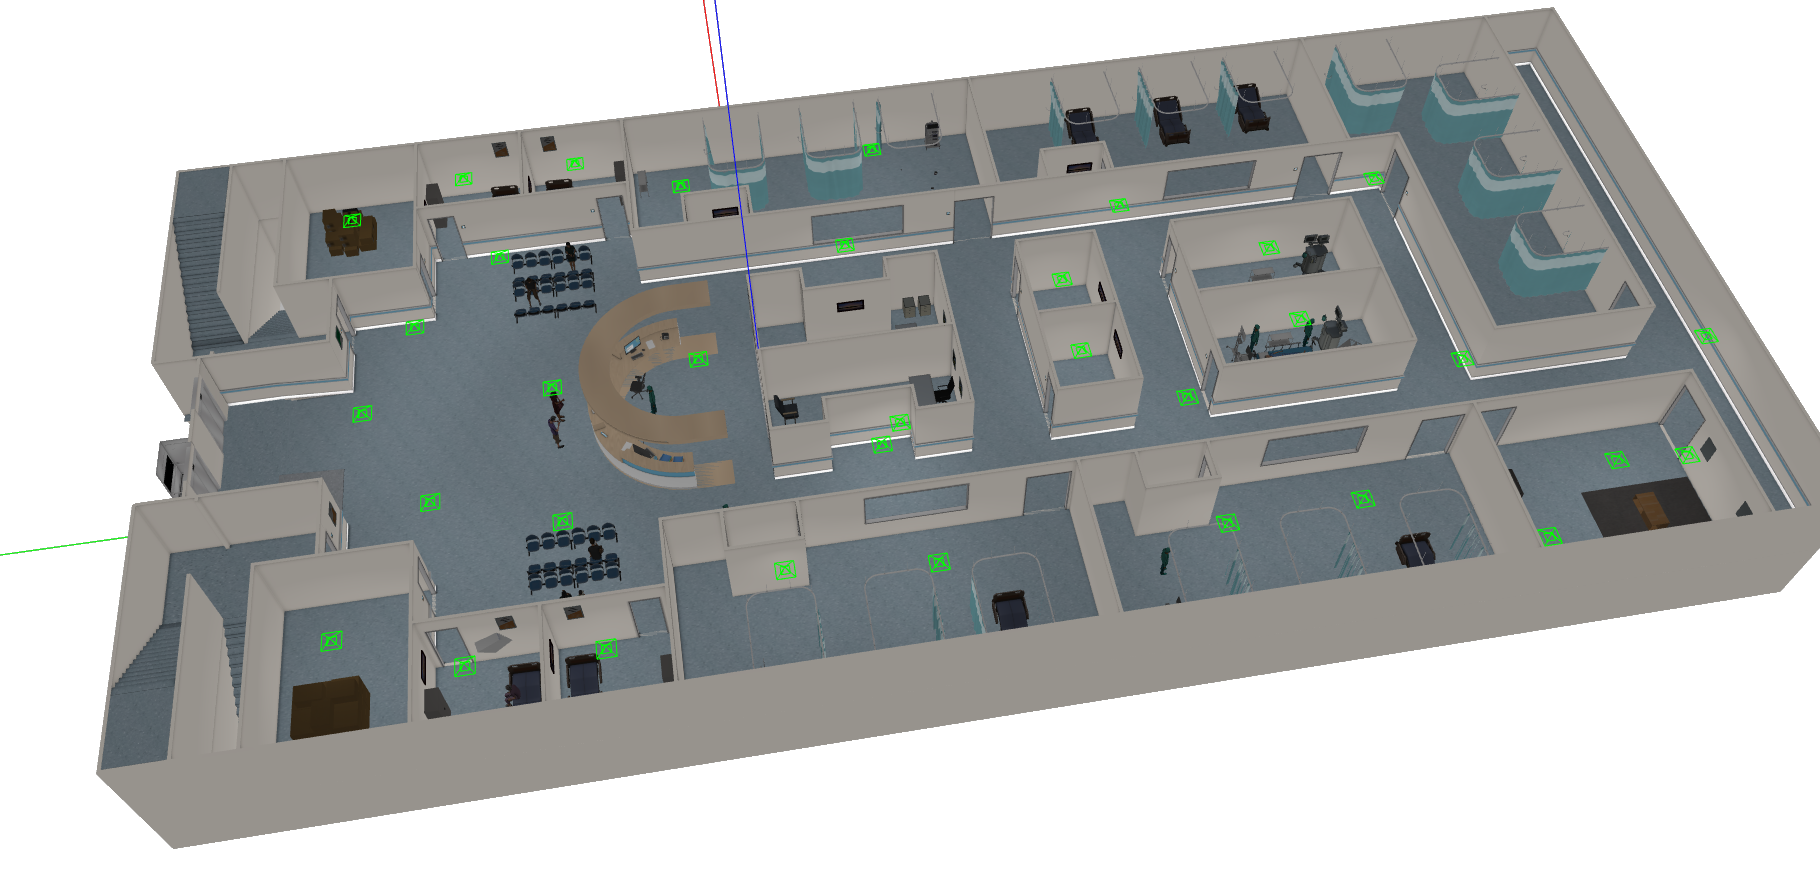
\includegraphics[width=0.8\textwidth]{Hospital.png}
    \caption{The hospital world environment [TODO ref]} \label{fig:hospitalWorld}
    % https://chowdera.com/2022/04/202204111258552961.html
\end{figure}

The algorithms were tested in each of the presented environments with several minutes long robot runs. The robot's trajectory was chosen so that the robot visits the same places several times to test the place recognition algorithm properly. All the robot runs were saved in rosbag files to ensure the repeatability of each experiment. Furthermore, every experiment for every metric presented further in this chapter has been performed on the same trajectory.\par
The dataset generated for the parameter tuning, described in the section \ref{section:parameterTuning}, and for the training of the neural networks, described in the section \ref{section:nnTraining}, were generated exclusively from the warehouse environment. The datasets' trajectory was entirely different from the trajectory used for the performance testing, but the type of the objects remained similar. In these datasets were no scenes from the other two environments.
\section{Evaluation}\label{section:Evaluation}

The result of a place recognition for a single scene can be either positive or negative. The positive evaluation means that the scene matched one of the previous ones, and the negative means that this scene is entirely new. However, in contrast to many classification algorithms, the result strongly depends on the earlier results, and the evaluation order of scenes matters. Furthermore, the classification algorithms generate the ids of the scenes instead of the direct positive/negative evaluation.\par
Let $n$ be number of scenes in the simulation and $S = \left(s_1, s_2, \dots, s_n\right)$ an ordered set of scenes that are gradually passed as an input to the algorithm. Let $P = \left(p_1, p_2, \dots, p_n\right)$ be an ordered set of the exact robot locations\footnote{$x$ and $y$ coordinates} and $O = \left(o_1, o_2, \dots, o_n\right)$ be an ordered set of exact robot orientations, on which the robot was in a time, when the appropriate scene was taken. Finally, let $R = \left(r_1, r_2, \dots, r_n \right)$ be an ordered set of scene ids, generated as an output of the place recognition algorithm.\par
Now, the result $r_i$ will be considered positive if
$$
    \exists j < i : r_j = r_i,
$$ and negative if
$$
    \forall j < i : r_j \neq r_i.
$$ The positive result is considered a false positive if the first scene with the same id is too far from the current scene in terms of location and orientation. The negative result is considered false negative if a previously saved scene is very close to the current scene in terms of location and orientation.\par
Formally, let
$$
    first\_ind(x) = \begin{cases}
        i\text{ st. } r_i = x \land \forall j < i: r_j \neq x & \text{ if $x \in R$} \\
        0                                                     & \text{ otherwise}    \\
    \end{cases}
$$
be a function that returns the index of the first scene evaluated with an id $x$. Let $r_i$ be a positive result. $r_i$ is a false positive if and only if
$$
    \| p_{first\_ind(r_i)} - p_i \| > th_\text{pos1} \lor | o_{first\_ind(r_i)} - o_i | > th_{\text{ori1}}.
$$\par
Now let $r_i$ be a negative result. $r_i$ is a false negative if and only if
$$
    \exists x < r_i:  \| p_{first\_ind(x)} - p_i \| \le th_\text{pos2} \land | o_{first\_ind(x)} - o_i | \le th_{\text{ori2}}.
$$\par
The thresholds depend on the resolution of the cell network used in the RatSLAM algorithm. Based on the robot's dimensions, the place cell size was chosen as 20 cm, slightly smaller than the robot. If the positively evaluated location is close enough, e.g., in the neighboring cells as the matched location, the algorithm still works well. Because of this, the false positive position threshold $th_\text{pos1}$ was chosen as 80 cm, which is more then four cells away. Similary, the size of orientation cells is 12°, and the false positive threshold $th_\text{pos2}$ was chosen as ca 22.9183°.\par
The false negative thresholds were chosen the same as the cell sizes, so 20 cm and 12°.

\section{System setup}\label{section:SystemSetup}

The system's performance has to be measured without influencing the program's run. This purpose serves the Node LVAnalyzer, which only subscribes to several topics and does not publish any messages. This node performs the complete performance analysis of the system.\par
This node contains a class Analyser, which performs the entire analysis. After the initialization, the class can be used by repeatedly calling its method insert. This method takes an id of a newly classified scene together with the robot's position and orientation at the scene's time. If the id is new, the position and orientation are stored, and all previously stored positions and orientations are compared to detect possible false negative. If the id already exists, the current position and orientation are compared with the stored one to detect possible false positive evaluation.\par
If the insert method is called on all scenes during the algorithm's run, the total number of true and false positives and a total number of true and false negatives is calculated. Furthermore, the analyzer generates detailed information, like ids, time, and exact positions of all false positive and negative evaluations. In addition to that, if the scene images are passed as a third optional parameter to the insert method, the Analyser will generate images of all false positive evaluations to see the difference between the wrongly matched views. This class also provides an animated live preview of all the scenes and their matches, as shown in the figure \ref{fig:analExample}.\par

\begin{figure}[htpb]
    \centering
    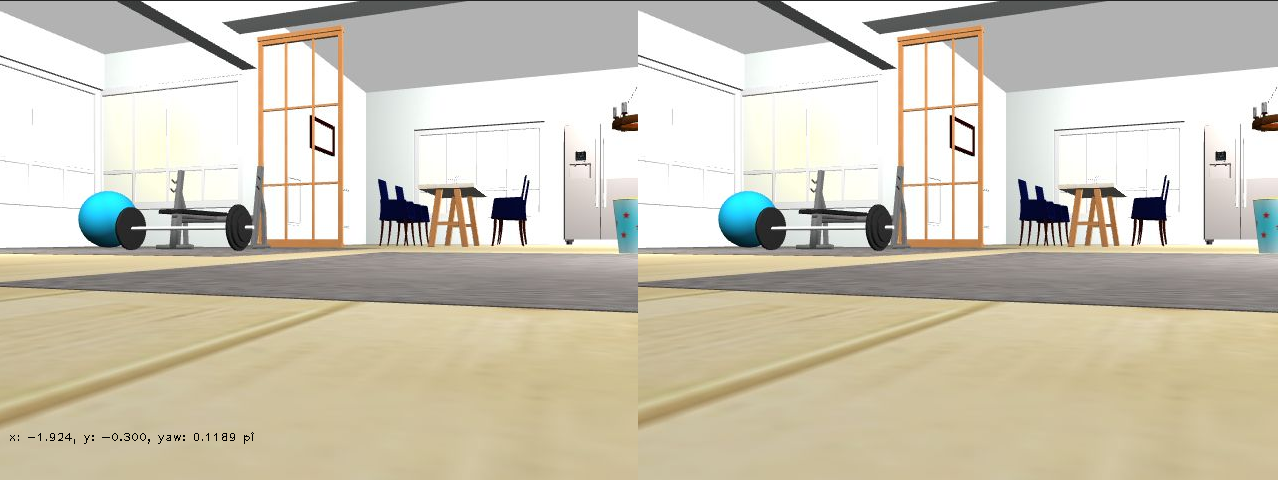
\includegraphics[width=0.8\textwidth]{analyserExample.png}
    \caption[Preview of the animation generated by the analyzer]{Preview of the animation generated by the analyzer. The left part shows a current scene and position, and the right part shows the preview of a matched scene.} \label{fig:analExample}
\end{figure}

The LVAnalyzer node is a wrapper over the Analyser class. This node subscribes to three topics, LVTemplate, Odometry, and Camera. After receiving a new matched template id from the LVTemplate topic, the exact position and scene image is found from the Odometry and Camera topics based on the timestamp of the messages. Afterward, all information is passed to the Analyser class using the insert method.

\section{Accuracy}\label{section:accuracy}

One of the essential evaluation metrics is the algorithm's accuracy, which will be measured in this section. In the beginning, the approaches presented in sections \ref{section:hierarchical} and \ref{section:2stage} will be compared using PR curves in all three environments. Afterward, the best thresholds will be picked, and the final accuracy measured for both approaches and compared with the accuracy of the visual matching used in the OpenRatSLAM.\par
The thresholds are one of the factors that influence the results the most. To find the best threshold values and to adequately compare both techniques, the accuracy, recall, and precision were measured for all possible threshold combinations with 0.01 steps. The measured values for all different thresholds were used to build the PR curves, presented in Figure \ref{fig:prCurves}.\par

\begin{figure}[!tbp]
    \centering
    \subfloat[Warehouse environment]{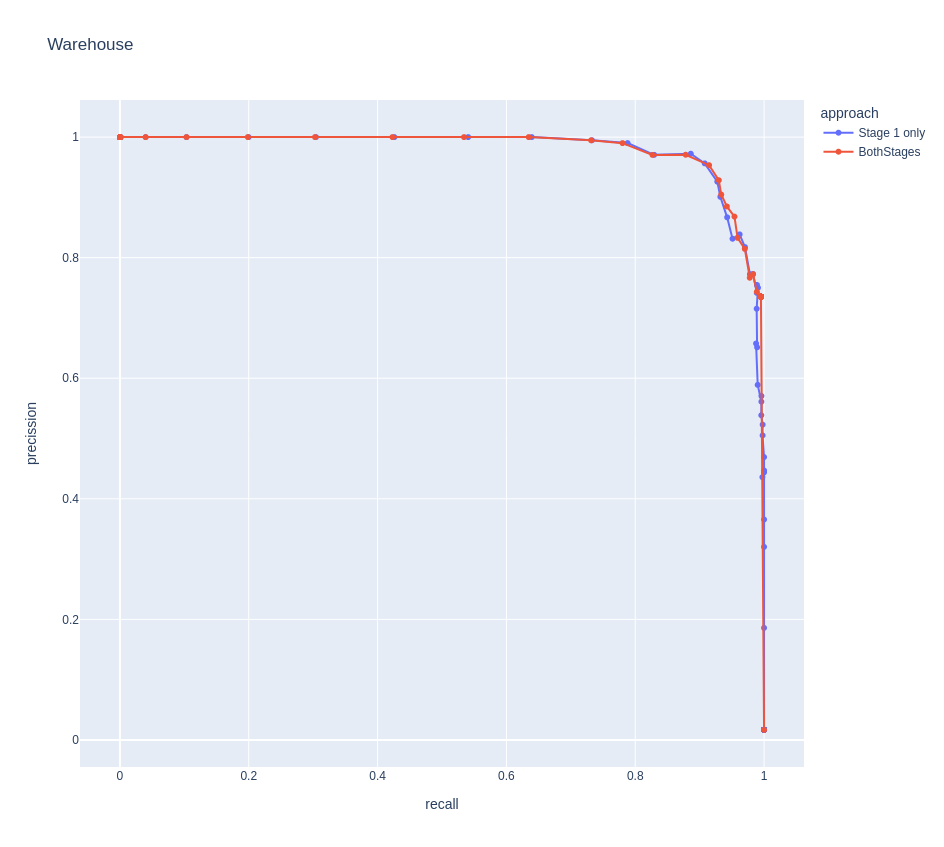
\includegraphics[height=0.3\textheight]{warehousePR.png}\label{fig:prCurvesWarehouse}}
    \hfill
    \subfloat[House environment]{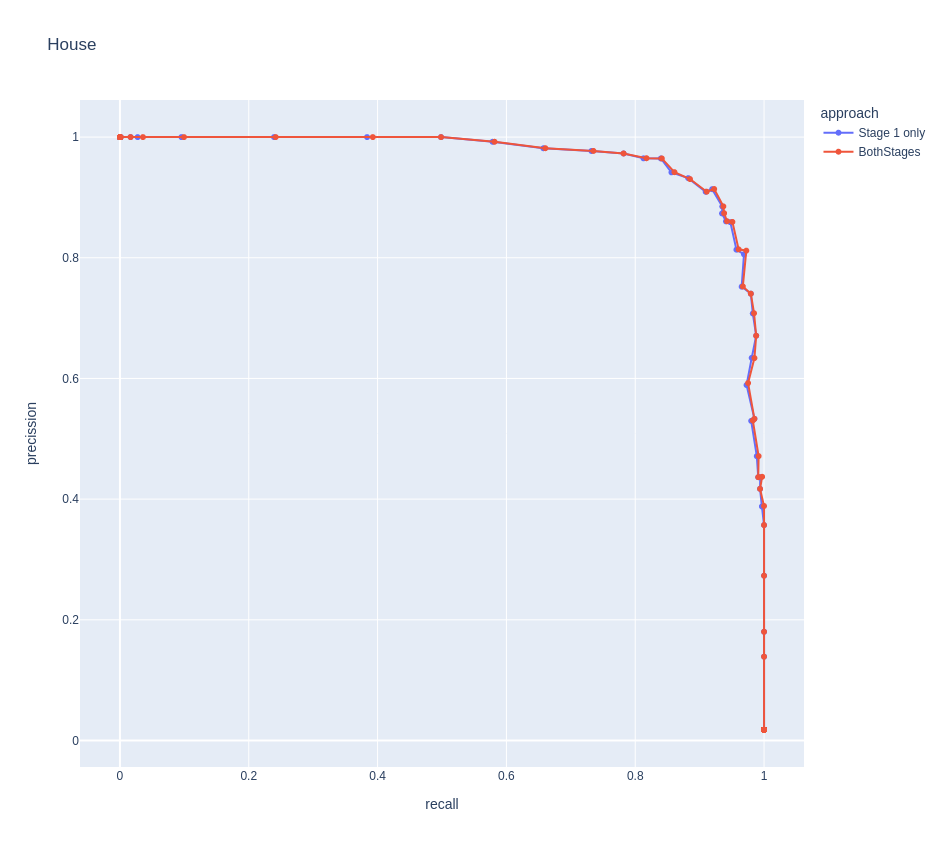
\includegraphics[height=0.3\textheight]{housePR.png}\label{fig:prCurveshouse}}
    \\
    \subfloat[Hospital environment]{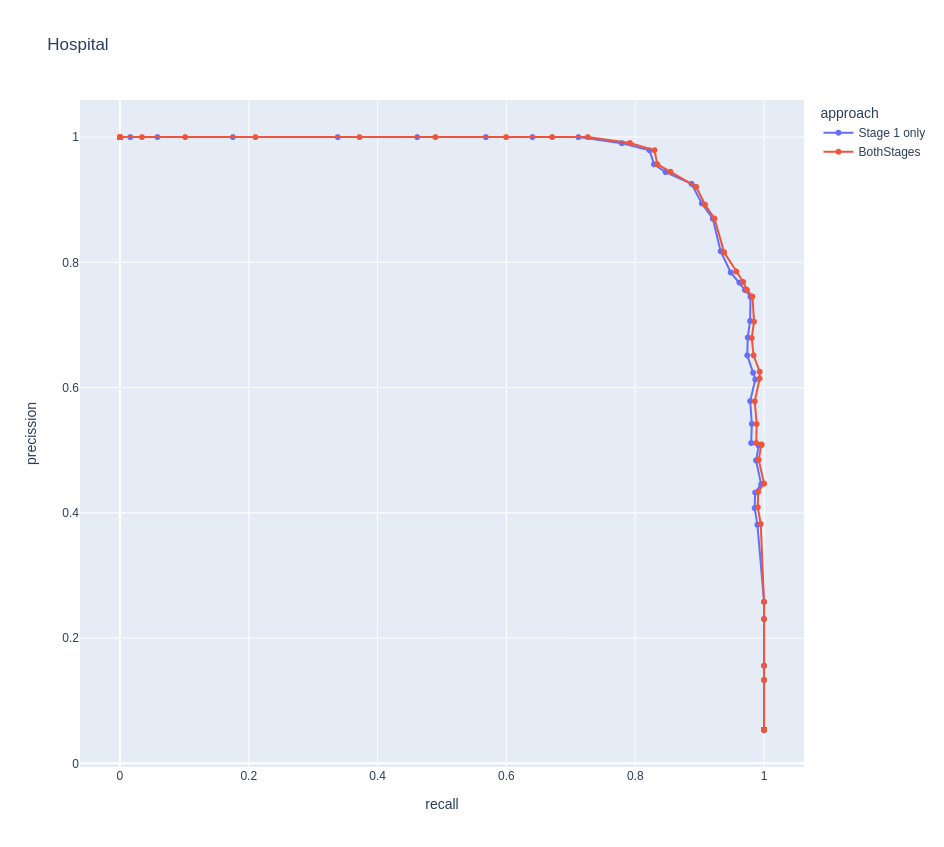
\includegraphics[height=0.3\textheight]{hospitalPR.png}\label{fig:prCurvesHospital}}
    \caption{PR Curves comparing Hierarchical and 2-Stage view matching approaches}
    \label{fig:prCurves}
\end{figure}


Because the thresholds influence only the LV matching part and not the LV building part, the local views were built and saved using the LV Dataset creator node, presented in section \ref{section:lvdatasetCreator}. This dataset was afterward used for evaluation instead of running the whole simulation, which saved a lot of time.\par
As Figure \ref{fig:prCurves} shows, both approaches have very similar results. Still, the method with two stages slightly outperforms the hierarchical approach with only the first stage by eliminating some false positive evaluations. Examples of false positives, evaluated by the first stage and eliminated by the second stage, are shown in Figure \ref{fig:eliminatedFPExamples}.\par

\begin{figure}[!tbp]
    \centering
    \subfloat{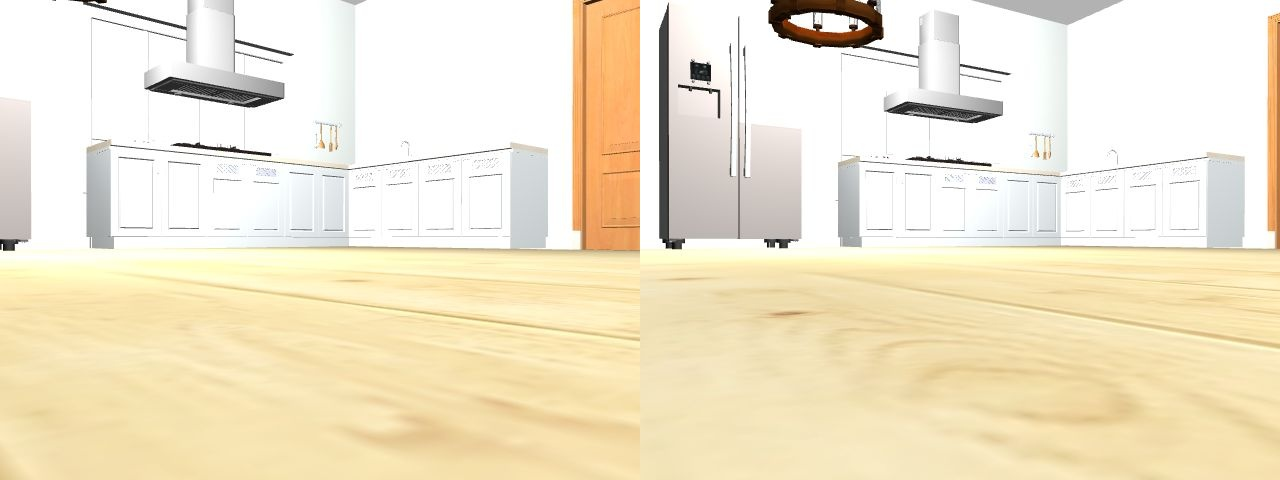
\includegraphics[width=0.8\textwidth]{eliminatedFPExample1.jpg}\label{fig:eFPEx1}}
    \\
    \subfloat{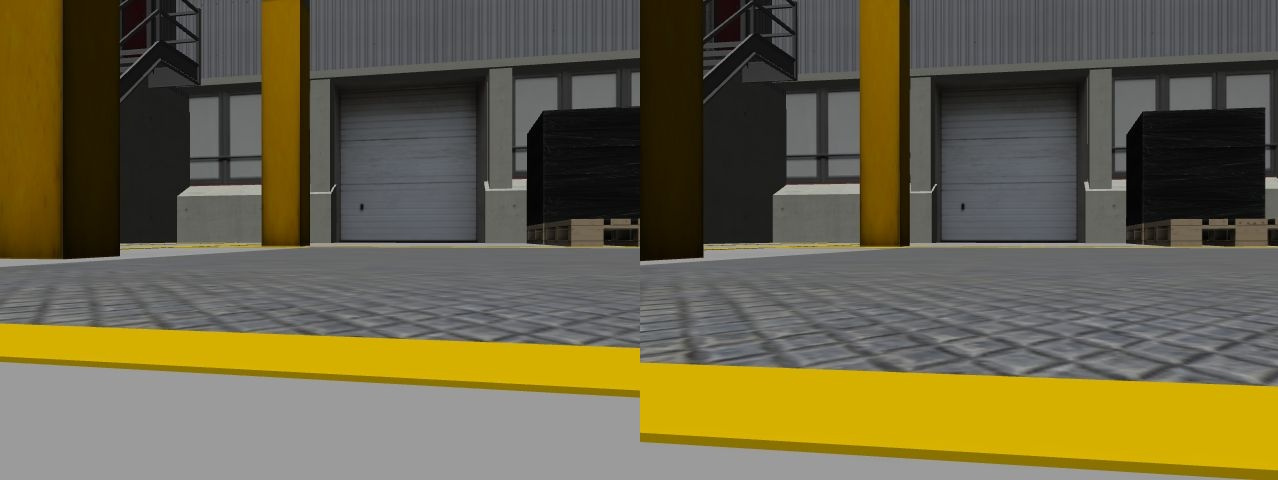
\includegraphics[width=0.8\textwidth]{eliminatedFPExample2.jpg}\label{fig:eFPEx2}}
    \caption{Examples of false positives eliminated by the second stage}
    \label{fig:eliminatedFPExamples}
\end{figure}

After the optimal thresholds were picked, the overall accuracy of both approaches was measured and compared with the accuracy of the visual place recognition used in the OpenRatSLAM. The results are shown in the table \ref{tab:accuracy}.

\begin{table}[htpb]
    \caption{Accuracy of all approaches in different environments}\label{tab:accuracy}
    \centering
    \begin{tabular}{l l l l}
        \toprule
        \textbf{}          & \textbf{1st stage only} & \textbf{both stages} & \textbf{OpenRatSLAM} \\
        \textbf{Warehouse} & 88.84 \%                & 89.28 \%             & 77.67 \%             \\
        \textbf{House}     & 86.69 \%                & 86.94 \%             & 41.25 \%             \\
        \textbf{Hospital}  & 86.19 \%                & 86.38 \%             & 79.36 \%             \\
        \bottomrule
    \end{tabular}
\end{table}

As the results show, both approaches have very similar results in all environments, but the method with both stages still slightly outperformed the technique with only the first stage. We can also see that both suggested approaches significantly outperformed the visual place recognition used in the OpenRatSLAM version in every environment, especially in the house world. Furthermore, the experiment results proved the ability to generalize on the environments diametrally different from the warehouse environment used for the model training.

\section{Average False Positive Error}\label{section:averageError}

Apart from the number of false positive and false negative evaluations, the distances of the false positives between the wrongly estimated scenes is another critical performance metric. If the false positive is close to the threshold and the distance is relatively small, then the result won't be influenced much. However, if the distance between wrongly matched scenes is very large, the negative impact on the result will be significant.\par
This section analyzes distances for every false positive result during the simulation in every environment. The exact distances for every false positive evaluation for both approaches are shown in figures \ref{fig:averageFPErrorWarehouse}, \ref{fig:averageFPErrorHouse}, and \ref{fig:averageFPErrorHospital}. The average and maximal error distance for each approach in each environment, together with the comparison with the visual place recognition used in the original RatSLAM, is shown in the table \ref{tab:averageFPError}.\par

\begin{figure}[!tbp]
    \centering
    \subfloat[1st stage only]{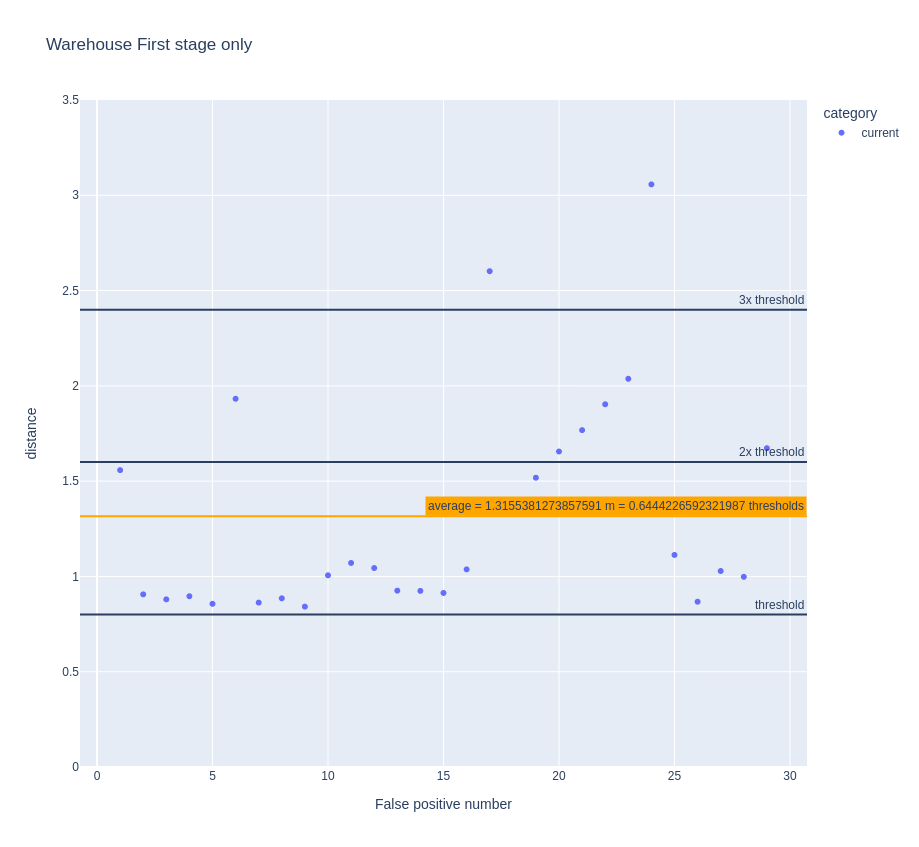
\includegraphics[width=0.5\textwidth]{warehouseFirstStageFalsePositiveDistances.png}\label{fig:FPErr11}}
    \hfill
    \subfloat[Both stages]{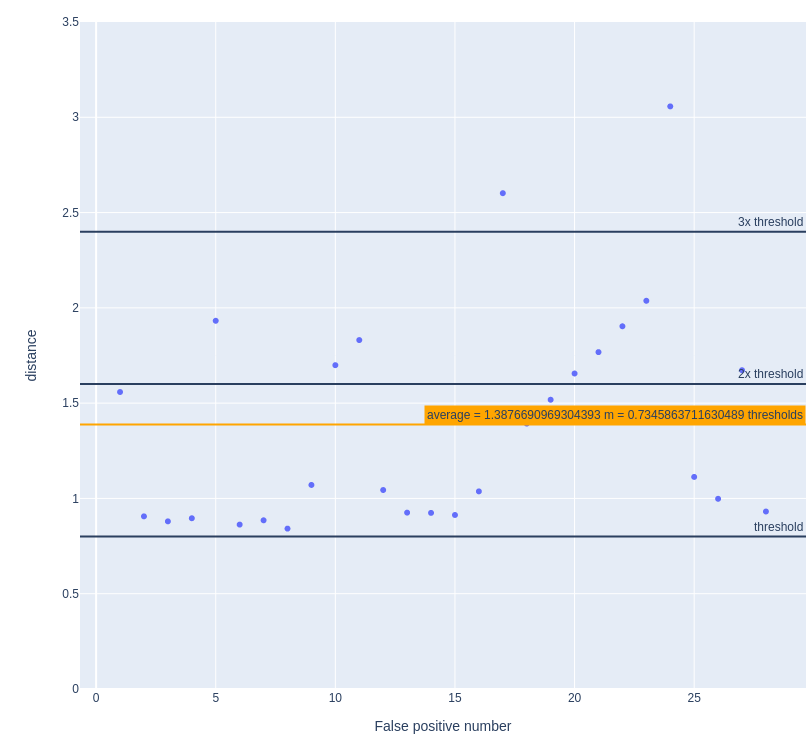
\includegraphics[width=0.5\textwidth]{warehouseBothStagesFalsePositiveDistances.png}\label{fig:FPErr12}}
    \caption{False positive distances in the warehouse environment}
    \label{fig:averageFPErrorWarehouse}
\end{figure}

\begin{figure}[!tbp]
    \centering
    \subfloat[1st stage only]{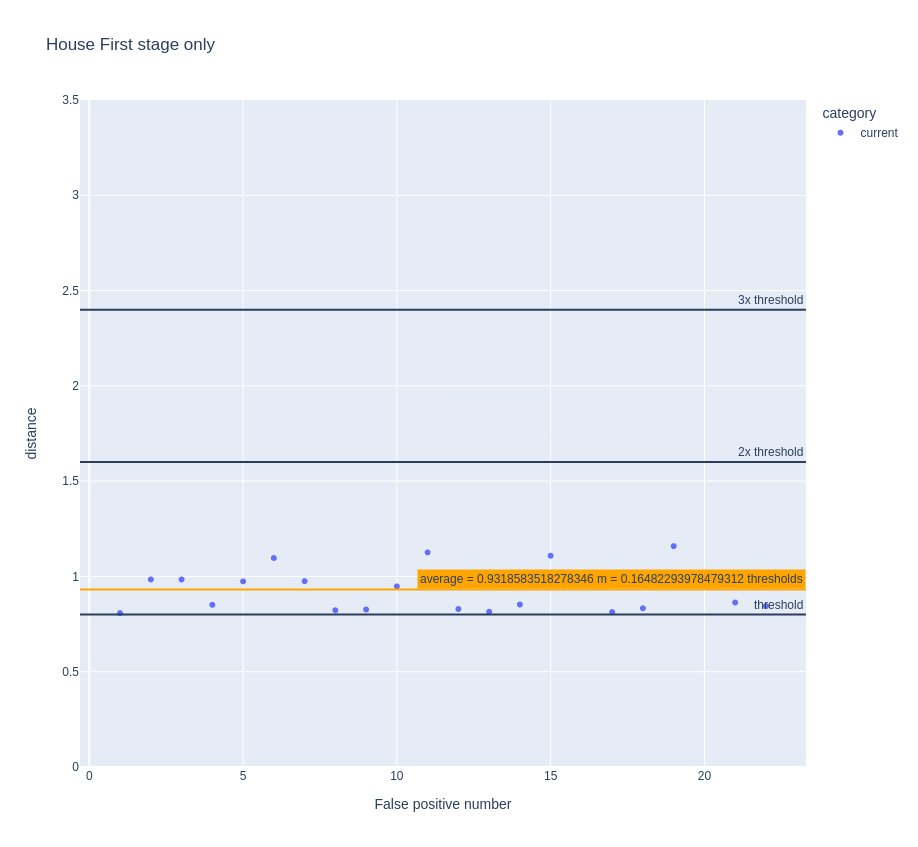
\includegraphics[width=0.5\textwidth]{houseFirstStageFalsePositiveDistances.png}\label{fig:FPErr21}}
    \hfill
    \subfloat[Both stages]{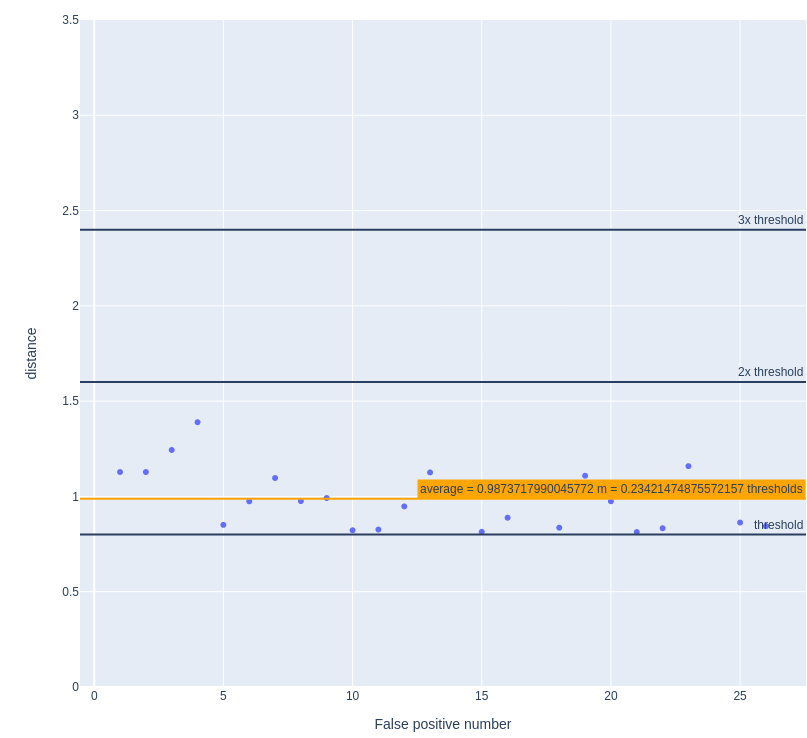
\includegraphics[width=0.5\textwidth]{houseBothStagesFalsePositiveDistances.png}\label{fig:FPErr22}}
    \caption{False positive distances in the house environment}
    \label{fig:averageFPErrorHouse}
\end{figure}

\begin{figure}[!tbp]
    \centering
    \subfloat[1st stage only]{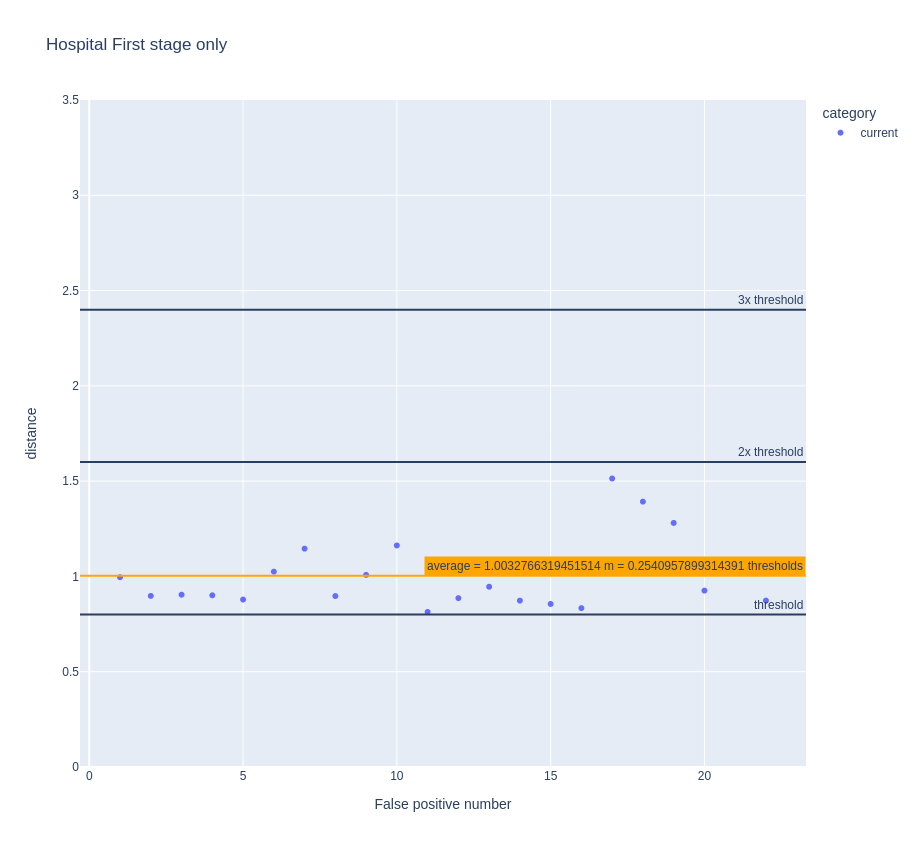
\includegraphics[width=0.5\textwidth]{hospitalFirstStageFalsePositiveDistances.png}\label{fig:FPErr31}}
    \hfill
    \subfloat[Both stages]{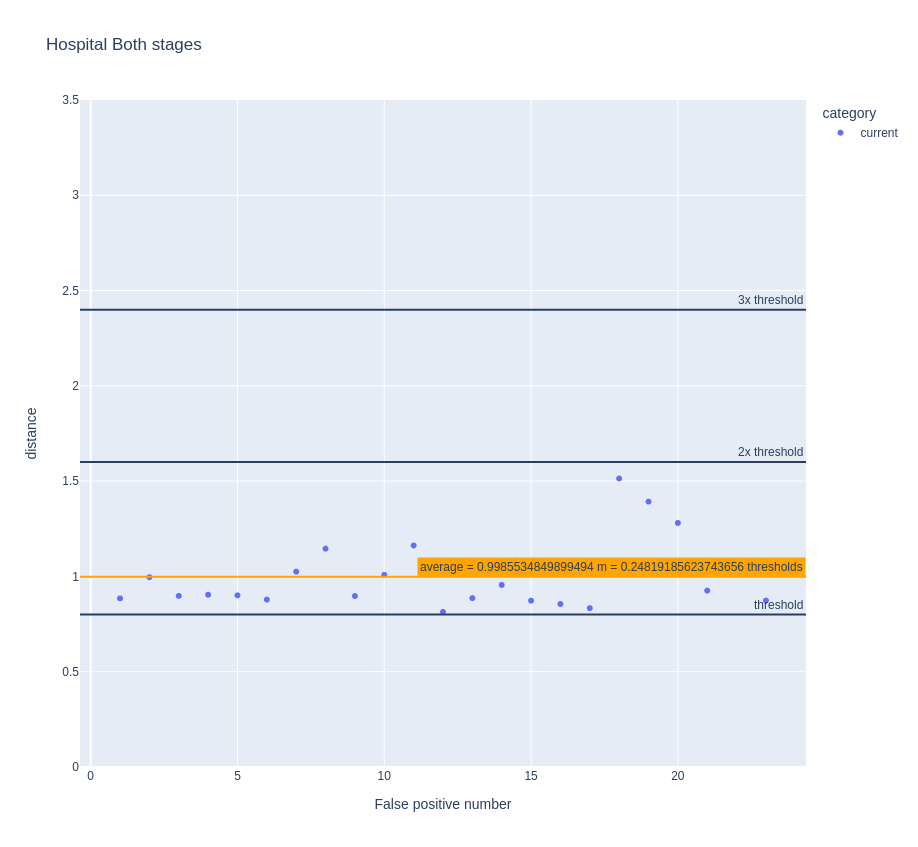
\includegraphics[width=0.5\textwidth]{hospitalBothStagesFalsePositiveDistances.png}\label{fig:FPErr32}}
    \caption{False positive distances in the hospital environment}
    \label{fig:averageFPErrorHospital}
\end{figure}

\begin{table}[htpb]
    \caption{Average and maximal errors of false positive evaluations in different environments}\label{tab:averageFPError}
    \centering
    \begin{tabular}{l | l  l| l l| l l}
        \toprule
        \textbf{}                      & \multicolumn{2}{l|}{\textbf{1st stage only}} & \multicolumn{2}{l|}{\textbf{both stages}} & \multicolumn{2}{l}{\textbf{original RatSLAM}}                             \\
        {}                             & avg                                          & max                                       & avg                                           & max    & avg    & max     \\
        \hline
        \textbf{Warehouse environment} & 1.32 m                                       & 3.06 m                                    & 1.39 m                                        & 3.06 m & 8.93 m & 11.52 m \\
        \textbf{House environment}     & 0.93 m                                       & 1.16 m                                    & 0.99 m                                        & 1.39 m & 1.84 m & 3.93 m  \\
        \textbf{Hospital environment}  & 1.00 m                                       & 1.52 m                                    & 1.00 m                                        & 1.51 m & 6.56 m & 14.57 m \\
        \bottomrule
    \end{tabular}
\end{table}

As the results show, both techniques suggested in this work showed outstanding performance in this metric. In the house and hospital environment, the average error lies only 13-20 cm away from the threshold, which is less than 25 \% of the threshold size. Moreover, all evaluated false negatives in these environments are not farther than twice the threshold from the matched scene. This means that all wrongly evaluated matches are still very close to the threshold and shouldn't cause almost any damage to the final result. Some errors in the warehouse environment were slightly larger, but they were only exceptional cases, and most of the wrongly classified matches are still very close to the threshold.\par
On the other hand, the results of the visual place recognition used in the original RatSLAM were significantly worse. As the results suggest, most of the wrongly evaluated scenes were spread over the whole environment, and the distances between the incorrectly matched scenes were huge. The most significant errors can be observed in the hospital environment, which drastically influenced the generated experience map, as discussed in the section \ref{section:RatSalmIntegration}.\par
According to this metric, both presented approaches significantly outperformed the visual place recognition used in the original RatSLAM.

\section{Time Performance}\label{section:timePerformance}

Another important property is the time of the local view template building and especially the time of comparing two templates. The time of the template building and comparing the two templates are measured separately. The reason is that the template building is done only once per scene, independently of the length of the algorithm's run. However, comparing the two templates is done more times for every scene. Namely, every new scene is compared with all previously saved scenes whose number increases over time, especially in large and various environments. Therefore, the time of the matching is the critical part and must be as fast as possible. In contrast, the time of the building can be significantly larger as long as it stays smaller than the period between two sensor inputs.\par
The system was tested on a Laptop with the following parameters:

\begin{description}[labelwidth=5em,leftmargin =\dimexpr\labelwidth+\labelsep\relax]
    \item[\textbf{Processor}:] Intel${}^{\text{\tiny{\textregistered}}}$ Core™ i7-8650U Processor (1.9 - 4.2 GHz) \footnote{\tiny{\url{https://ark.intel.com/content/www/us/en/ark/products/124968/intel-core-i7-8650u-processor-8m-cache-up-to-4-20-ghz.html}}}
    \item[\textbf{RAM}:]
          \begin{itemize}
              \item 4 GiB Row of chips DDR4 Synchronous Unbuffered (Unregistered) 2400 MHz (0,4 ns)
              \item 8 GiB SODIMM DDR4 Synchronous Unbuffered (Unregistered) 2400 MHz (0,4 ns)
          \end{itemize}
    \item[\textbf{OS}:] Kubuntu 21.10 x86\_64,
\end{description}

inside of the virtual machine, with the following limitations and operating system:

\begin{description}[labelwidth=5em]
    \item[\textbf{RAM}:] 8 GiB
    \item[\textbf{OS}:] Ubuntu 20.04 LTS x86\_64.
\end{description}

The GPU did not have CUDA support, so all the computations were performed on a CPU.\par
Figures \ref{fig:timesWarehouse}, \ref{fig:timesHouse}, and \ref{fig:timesHospital} show the LV building times for each scene and also matching times for each pair of compared scenes in all the environments. The table \ref{tab:averageTimes} shows the average times for each approach in every environment compared with the visual place recognition used in the OpenRatSLAM.


\begin{figure}[!tbp]
    \centering
    \subfloat[LV building times]{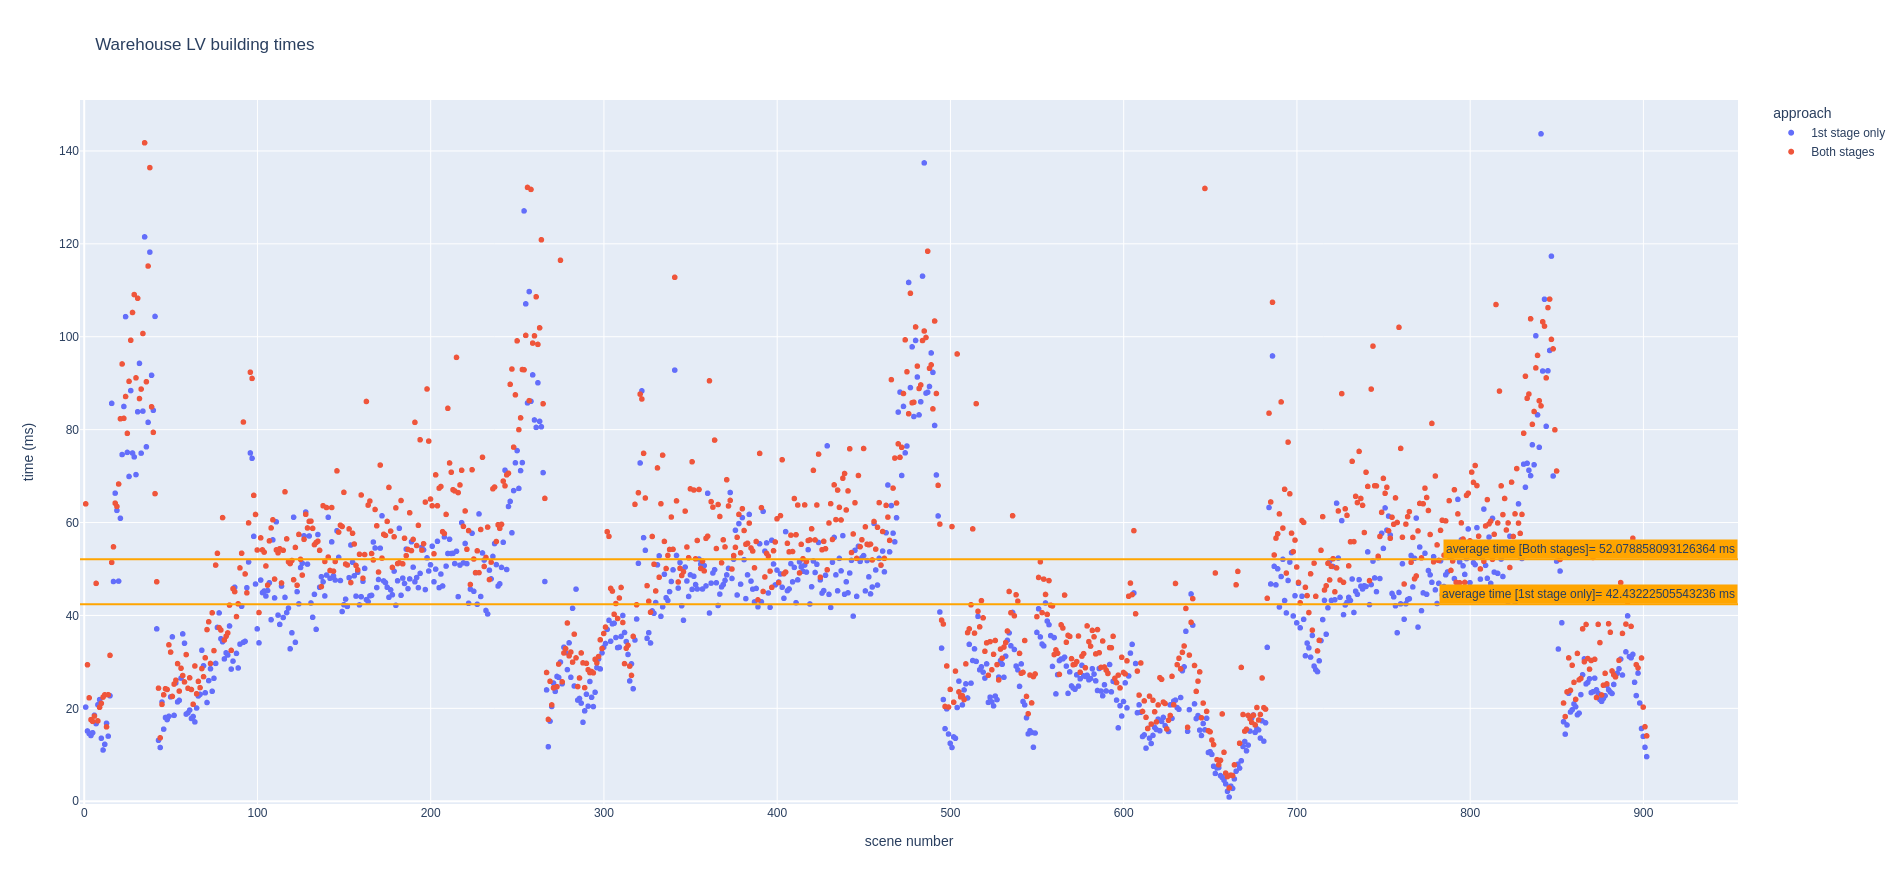
\includegraphics[width=0.8\textwidth]{warehouseBuildingTimes.png}\label{fig:timesWH1}}
    \\
    \subfloat[LV matching times]{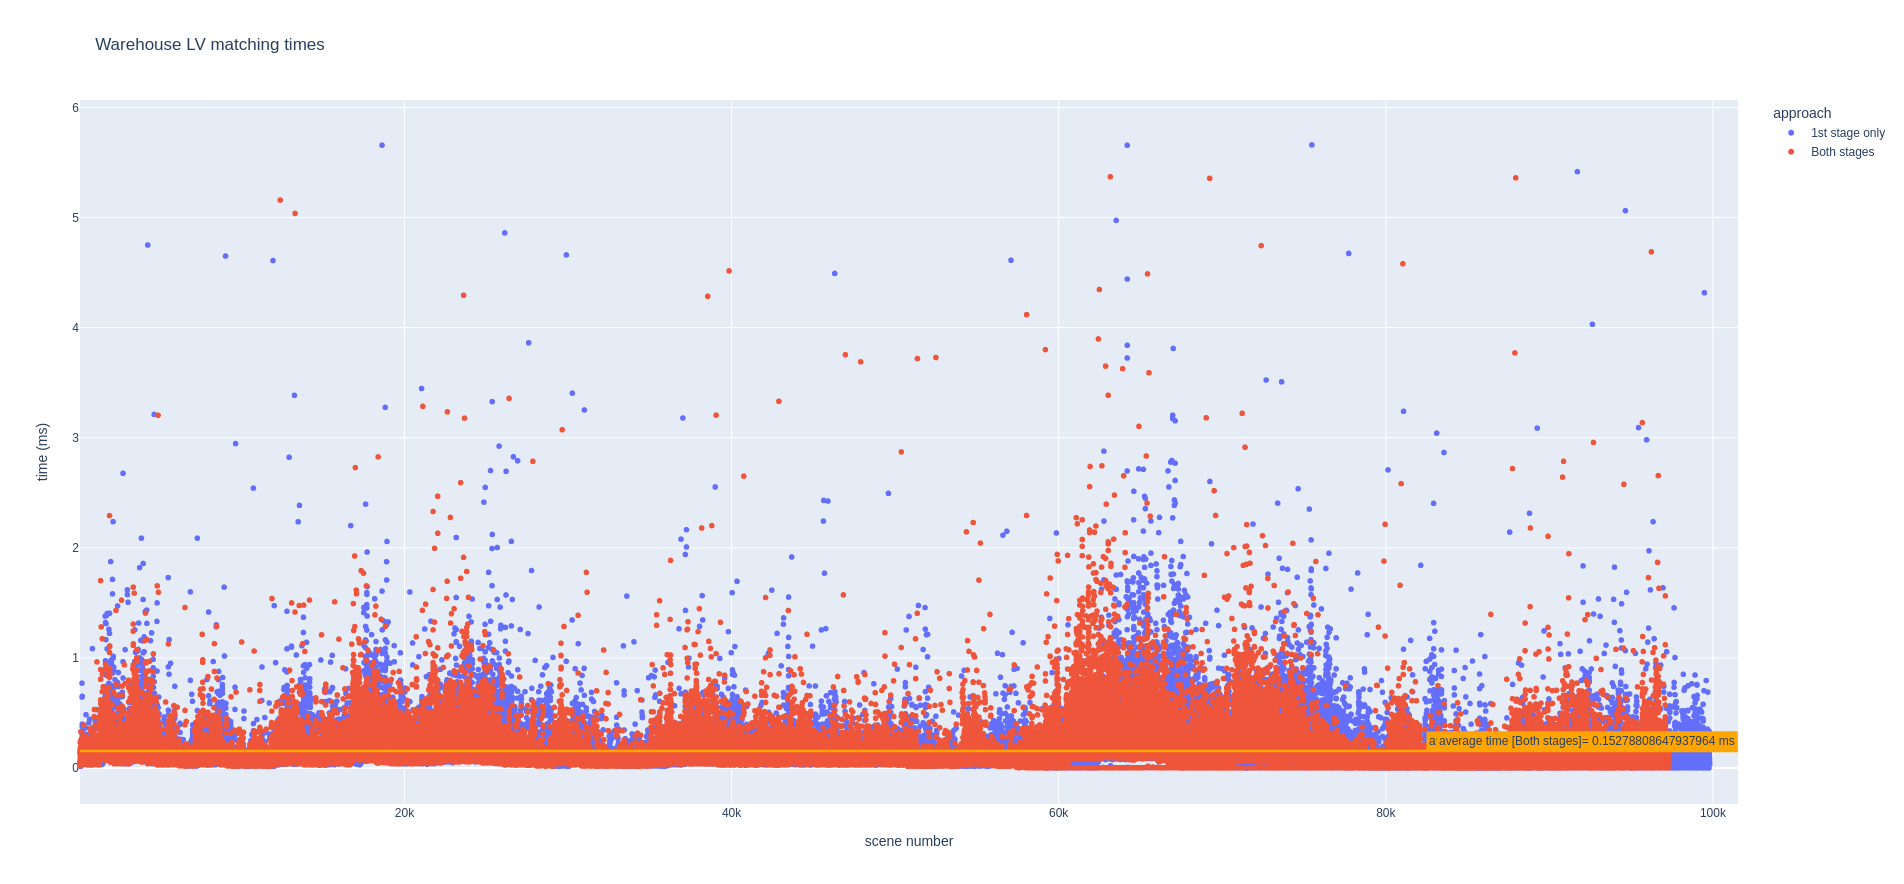
\includegraphics[width=0.8\textwidth]{warehouseMatchingTimes.png}\label{fig:timesWH2}}
    \caption{Computation times in the warehouse environment}
    \label{fig:timesWarehouse}
\end{figure}

\begin{figure}[!tbp]
    \centering
    \subfloat[LV building times]{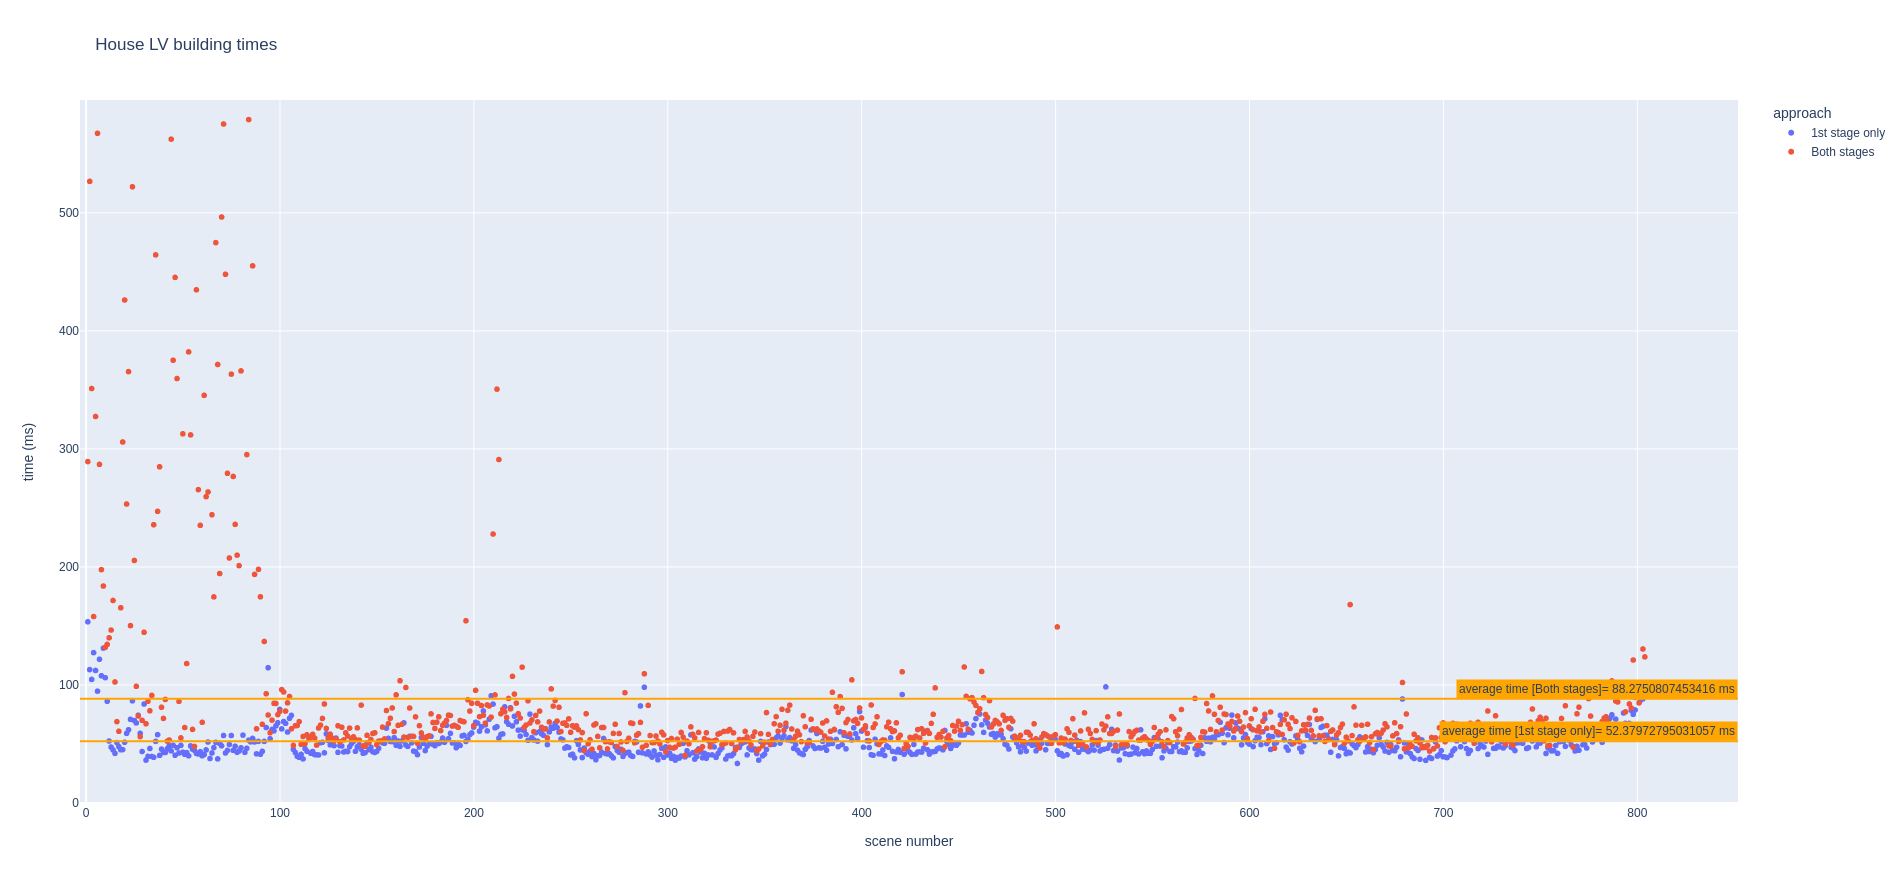
\includegraphics[width=0.8\textwidth]{houseBuildingTimes.png}\label{fig:timesHS1}}
    \\
    \subfloat[LV matching times]{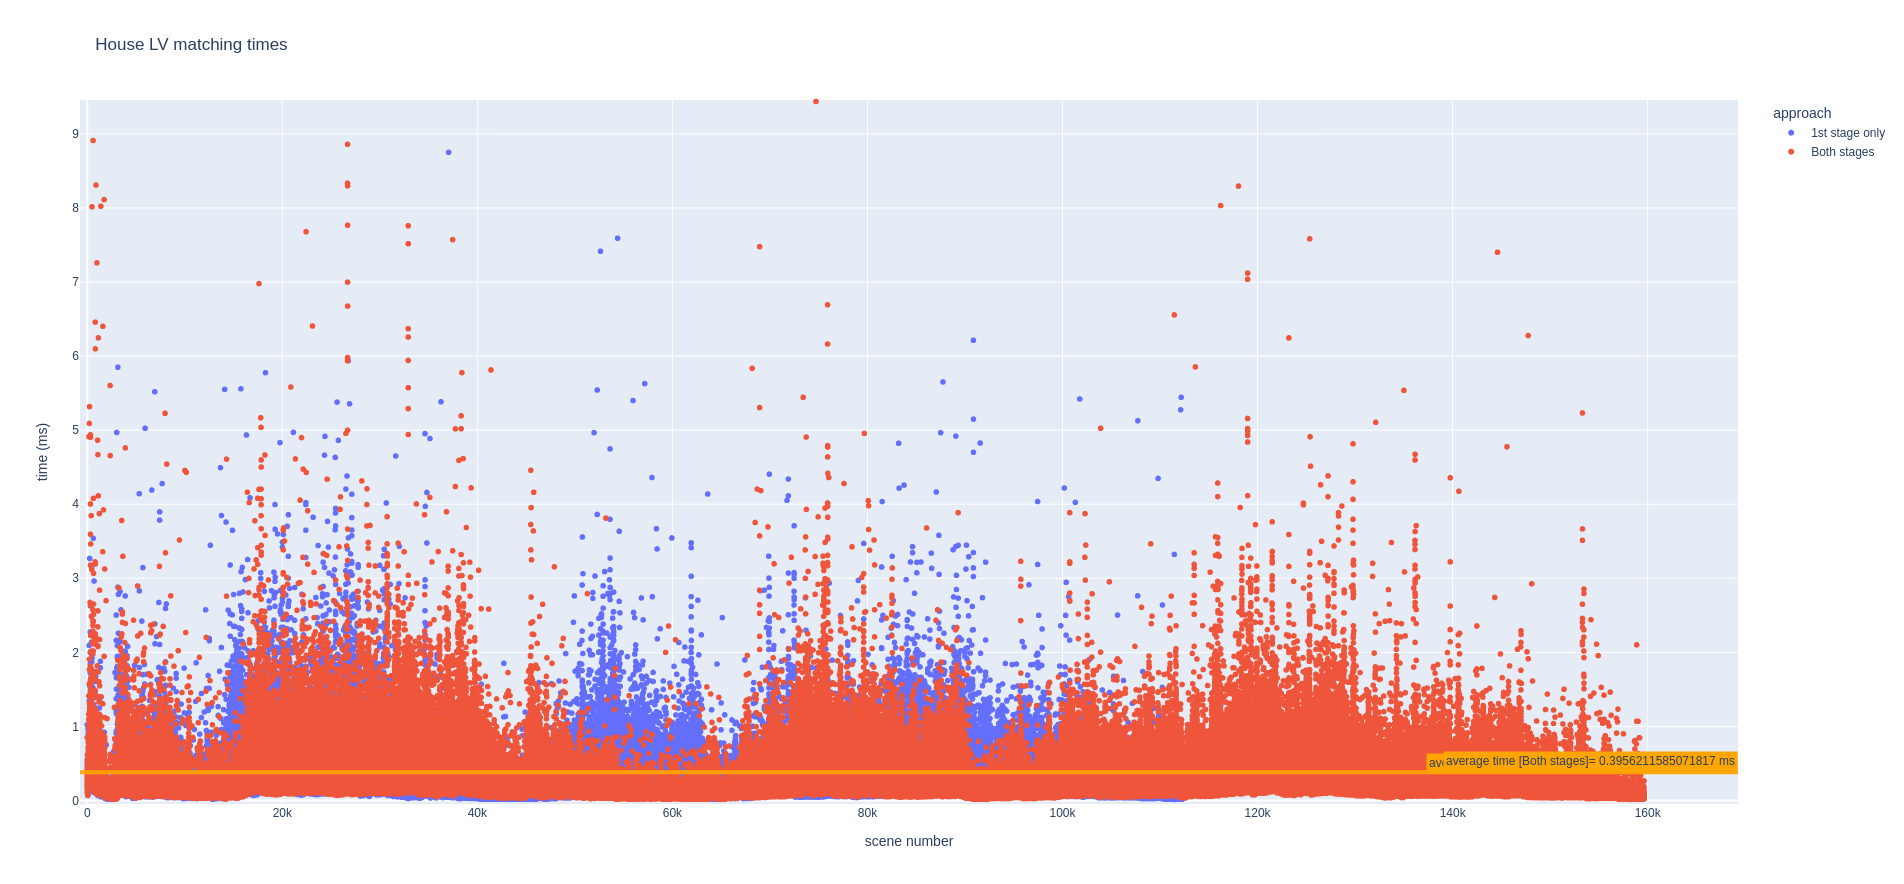
\includegraphics[width=0.8\textwidth]{houseMatchingTimes.png}\label{fig:timesHS2}}
    \caption{Computation times in the house environment}
    \label{fig:timesHouse}
\end{figure}

\begin{figure}[!tbp]
    \centering
    \subfloat[LV building times]{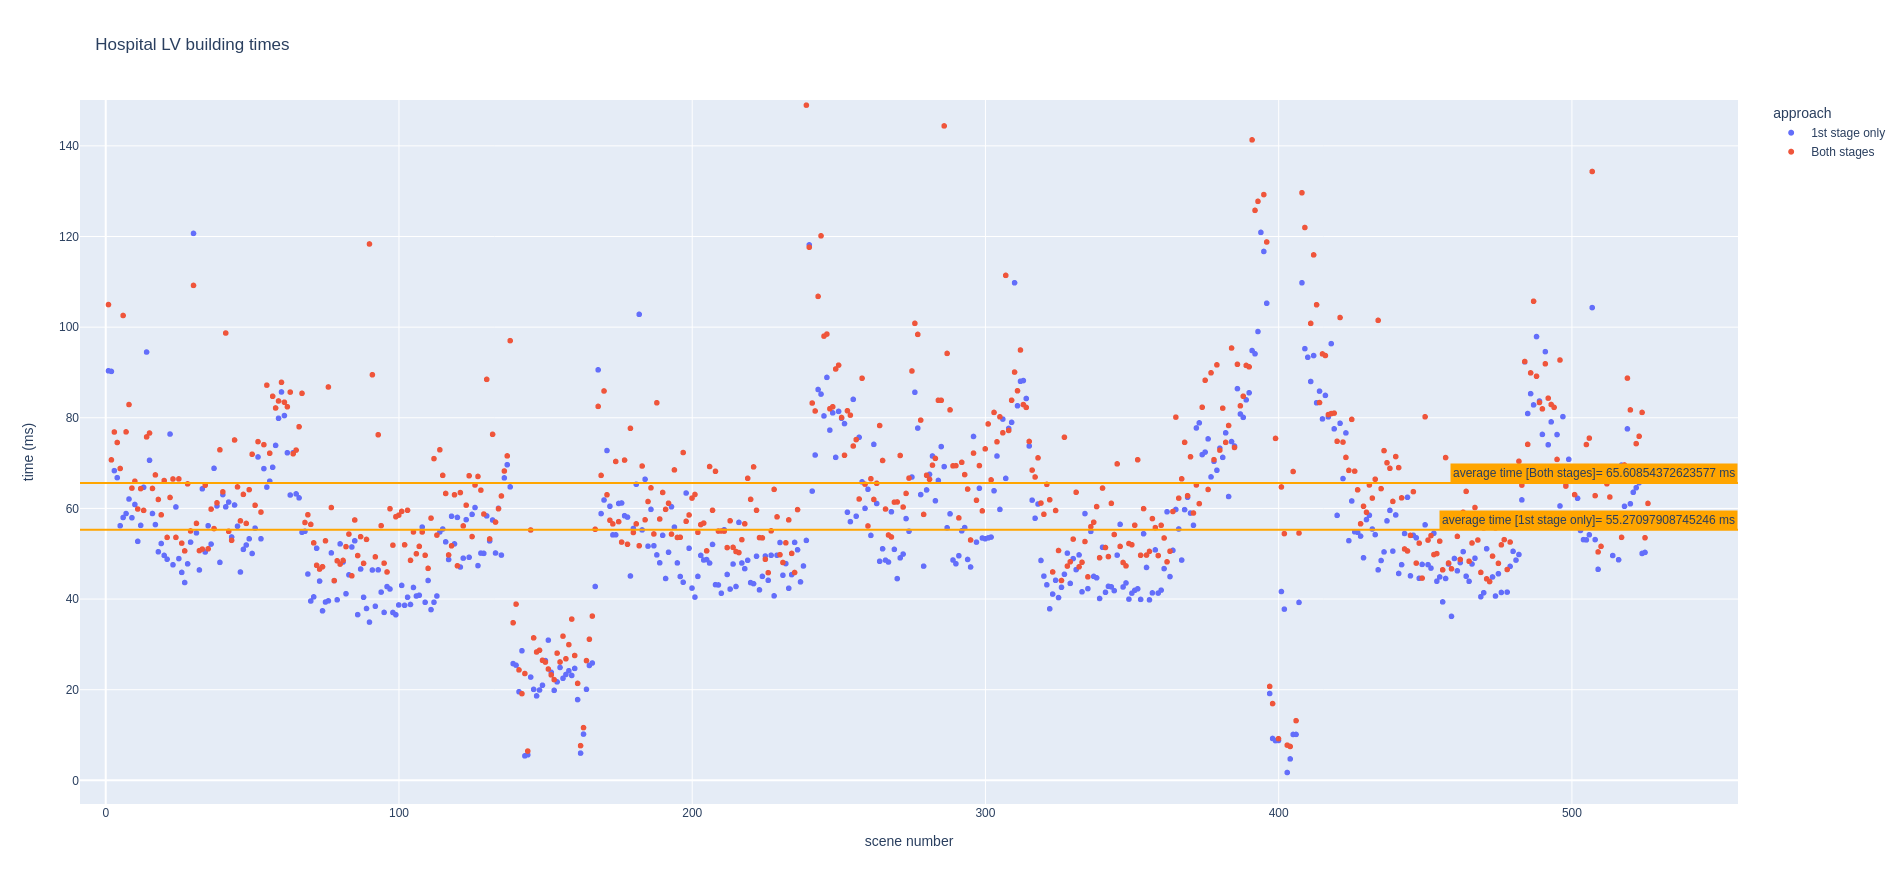
\includegraphics[width=0.8\textwidth]{hospitalBuildingTimes.png}\label{fig:timesHO1}}
    \\
    \subfloat[LV matching times]{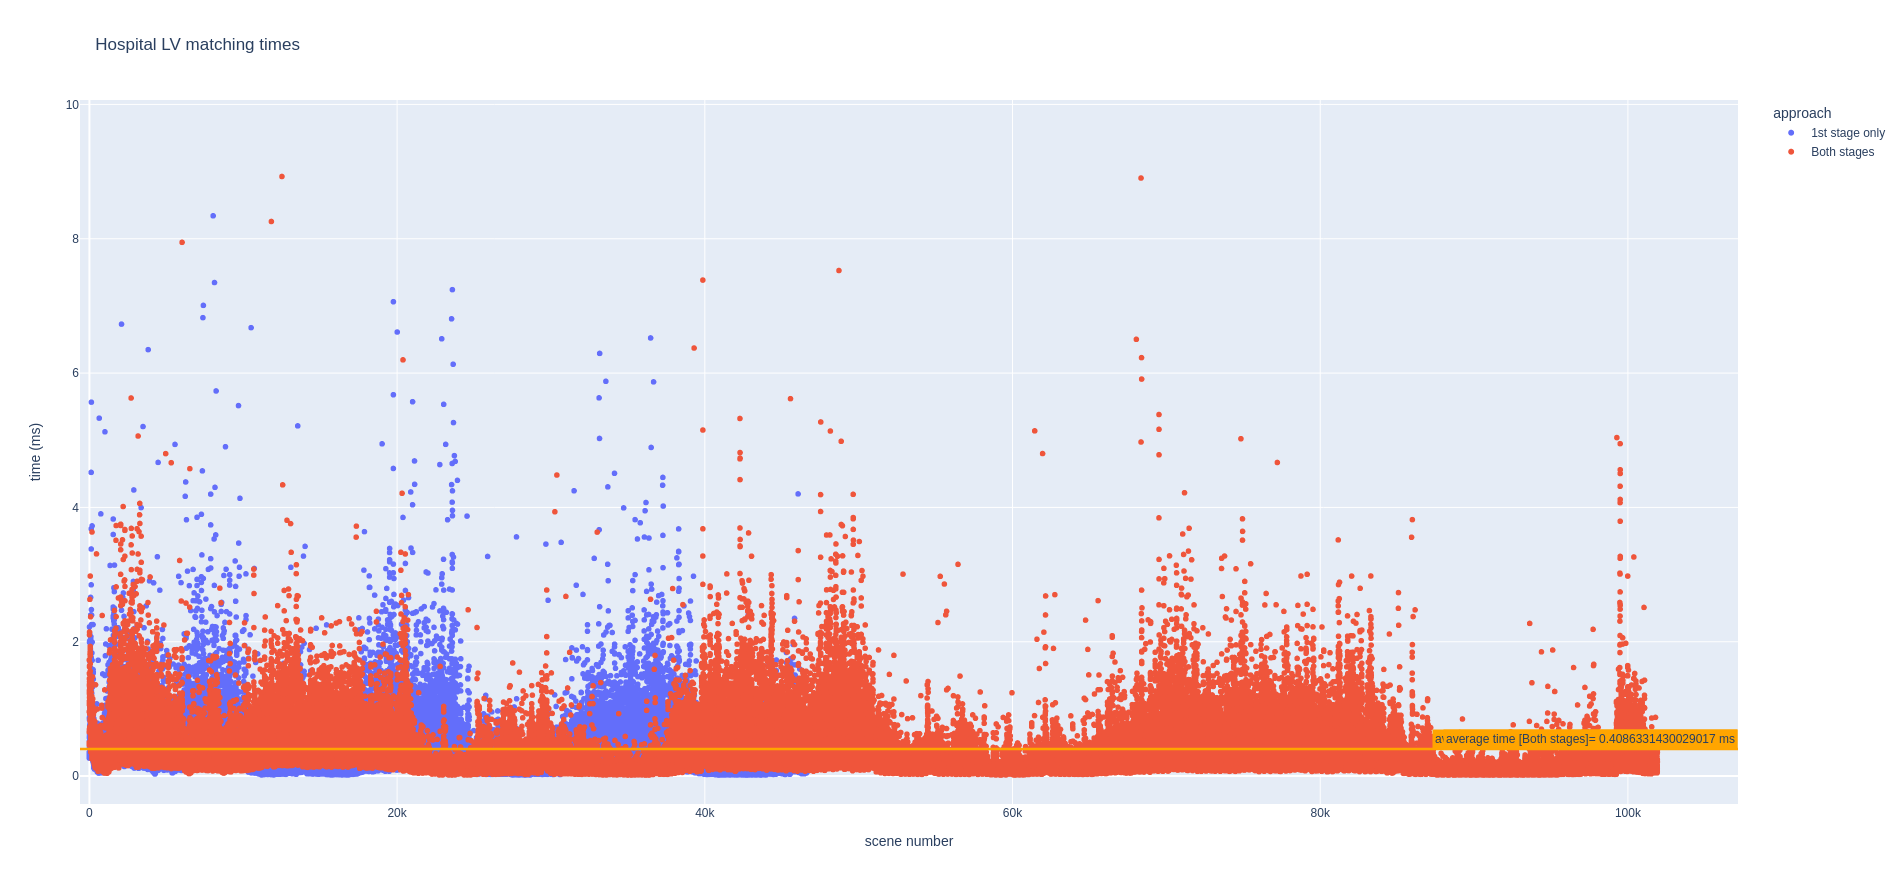
\includegraphics[width=0.8\textwidth]{hospitalMatchingTimes.png}\label{fig:timesHO2}}
    \caption{Computation times in the hospital environment}
    \label{fig:timesHospital}
\end{figure}

\begin{table}[htpb]
    \caption{Average times of LV matching and building in the different environments}\label{tab:averageTimes}
    \centering
    \begin{tabular}{l | l  l| l l| l l}
        \toprule
        \textbf{}          & \multicolumn{2}{l|}{\textbf{1st stage only}} & \multicolumn{2}{l|}{\textbf{both stages}} & \multicolumn{2}{l}{\textbf{OpenRatSLAM}}                                  \\
        {}                 & build                                        & match                                     & build                                    & match    & build    & match    \\
        \hline
        \textbf{Warehouse} & 42.432 ms                                    & 0.153 ms                                  & 52.078 ms                                & 0.159 ms & 2.053 ms & 0.083 ms \\
        \textbf{House}     & 52.380 ms                                    & 0.396 ms                                  & 88.265 ms                                & 0.368 ms & 1.448 ms & 0.137 ms \\
        \textbf{Hospital}  & 55.271 ms                                    & 0.399 ms                                  & 65.609 ms                                & 0.409 ms & 1.762 ms & 0.092 ms \\
        \bottomrule
    \end{tabular}
\end{table}

The table and graphs show that the approach that uses only the first stage can build the local views considerably faster than the 2-stage approach. The time difference is caused by the feature extraction, which is present only in the 2-stage approach. However, the time difference is not so significant. Most importantly, the techniques are significantly faster than the frequency of the sensors, so the time performance of local view building of both methods is satisfactory. As we can see, the LV building is significantly slower than the LV building in the OpenRatSLAM. However, the OpenRatSLAM works with sensors with significantly higher frequency\footnote{In the experiments, the frequency of the camera was 15 times higher than frequency of the LiDAR.}, so the LV building is done significantly more often, and the total resources consumption of the LV building process is comparable with the total consumption of the approaches presented in this work.\par
The times of the view matching of both approaches are almost the same, so the overhead caused by feature comparison in the second stage is practically negligible. Even if the times are circa 2 to 4 times larger than the times measured by the OpenRatSLAM, the number of saved views is significantly smaller, as shown in table \ref{tab:memory}, so the total comparison time for each scene will be at the end smaller than in the OpenRatSLAM approach. Furthermore, the times are significantly smaller than 1 ms, so there could be saved up to a thousand different local views to compare until the total comparison time reaches the sensors period. This means that this approach will also be suitable for very long time runs in huge environments.

\section{Memory Consumption}\label{section:memoryConsumption}

Especially for the robots with low-performant controllers, for example, older Raspberry PI, RAM is a very limited resource, so the memory needed for storing the local views needs to be as small as possible. Therefore another metric evaluated in the algorithms is the consumption of the memory. The measurement results are shown in the table \ref{tab:memory}.\par

\begin{table}[htpb]
    \caption{Average memory consumption of the algorithms in the different environments}\label{tab:memory}
    \centering
    \begin{tabular}{l | l  l| l l| l l}
        \toprule
        \textbf{}          & \multicolumn{2}{l|}{\textbf{1st stage only}} & \multicolumn{2}{l|}{\textbf{both stages}} & \multicolumn{2}{l}{\textbf{original RatSLAM}}                                                             \\
        {}                 & $\oslash$ LV size                            & $\oslash$ LVs stored                      & $\oslash$ LV size                             & $\oslash$ LVs st. & $\oslash$ LV size & $\oslash$ LVs st. \\
        \hline
        \textbf{Warehouse} & 78 B                                         & 194                                       & 1102 B                                        & 191               & 600 B             & 312               \\
        \textbf{House}     & 128 B                                        & 219                                       & 1152 B                                        & 216               & 600 B             & 445               \\
        \textbf{Hospital}  & 130 B                                        & 151                                       & 1154 B                                        & 148               & 600 B             & 219               \\
        \bottomrule
    \end{tabular}
\end{table}

The original RatSLAM uses a compressed 60x10 pixels big grayscale image as a local view template, so the memory needed for storing a single local view is always constant. However, the memory required for storing a single LV in the approaches suggested in this work differs for each local view and depends on the number of clusters detected by the DBScan algorithm. The difference between the size of the LV templates used in the approach with only the first stage and with both stages differs by a feature vector of 256 floating point numbers. Therefore, as follows from the table, the memory consumption of the first stage-only approach is significantly smaller than while also using the second stage.\par
The memory needed for storing the local views using the 2-stage approach is, on average, almost twice as large as the memory required for storing the lv template in the original RatSLAM approach. However, the number of stored templates in the original RatSLAM is almost twice larger than the number of stored templates in the 2-stage approach, so the total memory consumption remains similar. More interesting is the algorithm with only the first stage, in which a single local view consumes about six times less memory than the original RatSLAM approach. Furthermore, this approach stored, on average, significantly fewer local views than the original RatSLAM algorithm, so the total memory consumption is up to 12 times lower than in the original RatSLAM.

\section{RatSLAM Integration}\label{section:RatSalmIntegration}

The last metric to test is the integration with the RatSLAM. This section will integrate the scene recognition algorithm with the RatSLAM ROS system, generating the final experience maps. Finally, the maps generated for both approaches will be compared with the exact trajectory generated by the simulator and the experience map generated by the OpenRatSLAM with only visual scene recognition.\par
Even if the other evaluation techniques proved the significantly better performance of the methods suggested in this work, it is unclear if they will produce satisfactory results in connection with the RatSLAM, primarily because of the significantly lower frequency of the sensors. Therefore, this section aims to show that the improved performance compensates for the frequency loss of the sensors and that the generated results are at least as good as the results produced by the OpenRatSLAM or even better.\par

\begin{figure}[!tbp]
    \centering
    \subfloat[1st Stage only approaches]{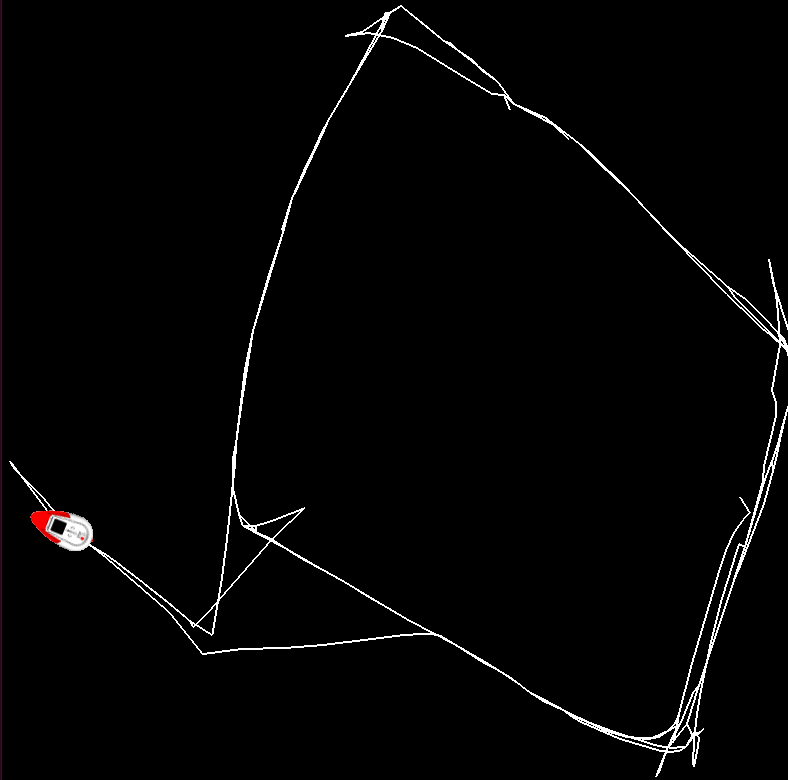
\includegraphics[height=0.3\textheight]{warehouse-1stStage.png}\label{fig:mapsWarehouse1st}}
    \hfill
    \subfloat[Both stages approaches]{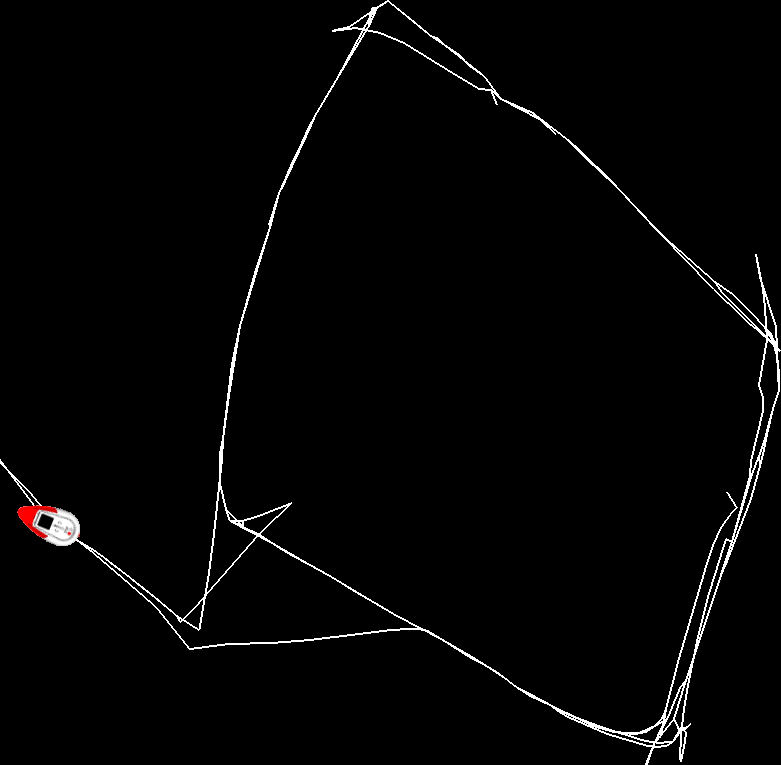
\includegraphics[height=0.3\textheight]{warehouse-bothStages.png}\label{fig:mapsWarehouseBot}}
    \\
    \subfloat[OpenRatSLAM]{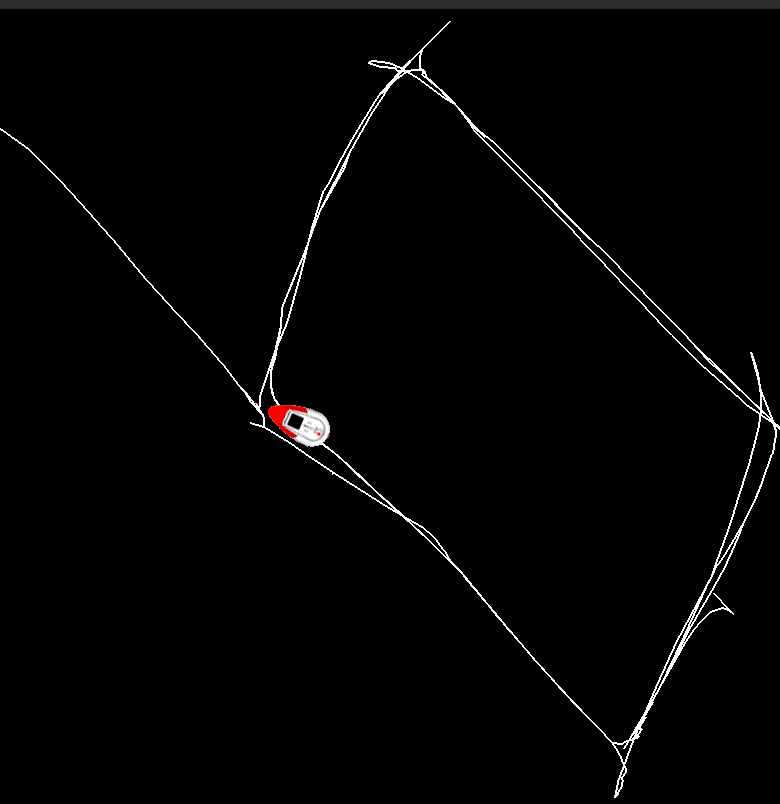
\includegraphics[height=0.3\textheight]{warehouse-ratslam.png}\label{fig:mapsWarehouseRat}}
    \hfill
    \subfloat[Exact trajectory]{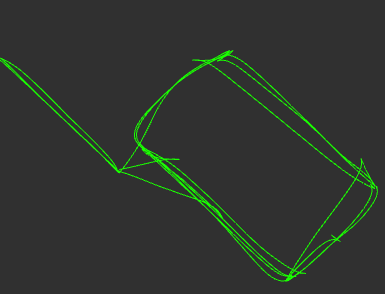
\includegraphics[height=0.3\textheight]{warehouse-exact.png}\label{fig:mapsWarehouseEx}}
    \caption{Generated experience maps in the warehouse environment}
    \label{fig:mapsWarehouse}
\end{figure}

\begin{figure}[!tbp]
    \centering
    \subfloat[1st Stage only approaches]{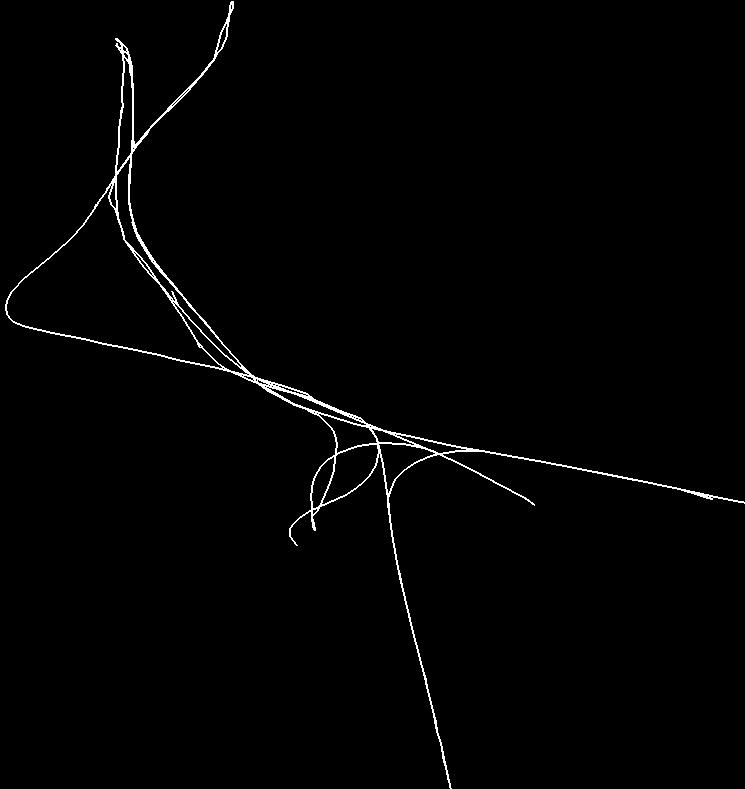
\includegraphics[height=0.3\textheight]{house-1stStage.png}\label{fig:mapsHouse1st}}
    \hfill
    \subfloat[Both stages approaches]{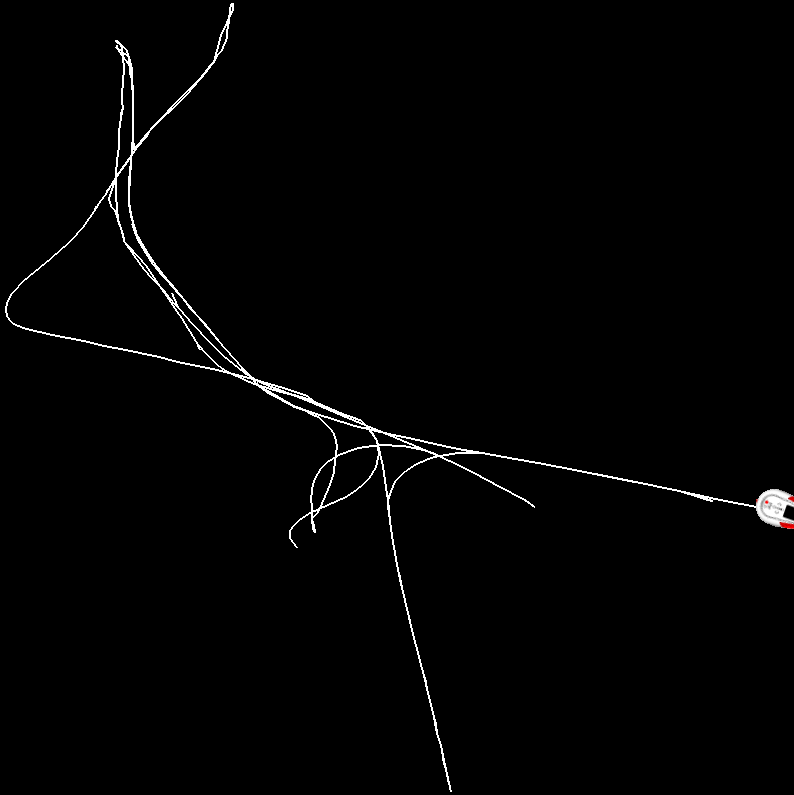
\includegraphics[height=0.3\textheight]{house-bothStages.png}\label{fig:mapsHouseBot}}
    \\
    \subfloat[OpenRatSLAM]{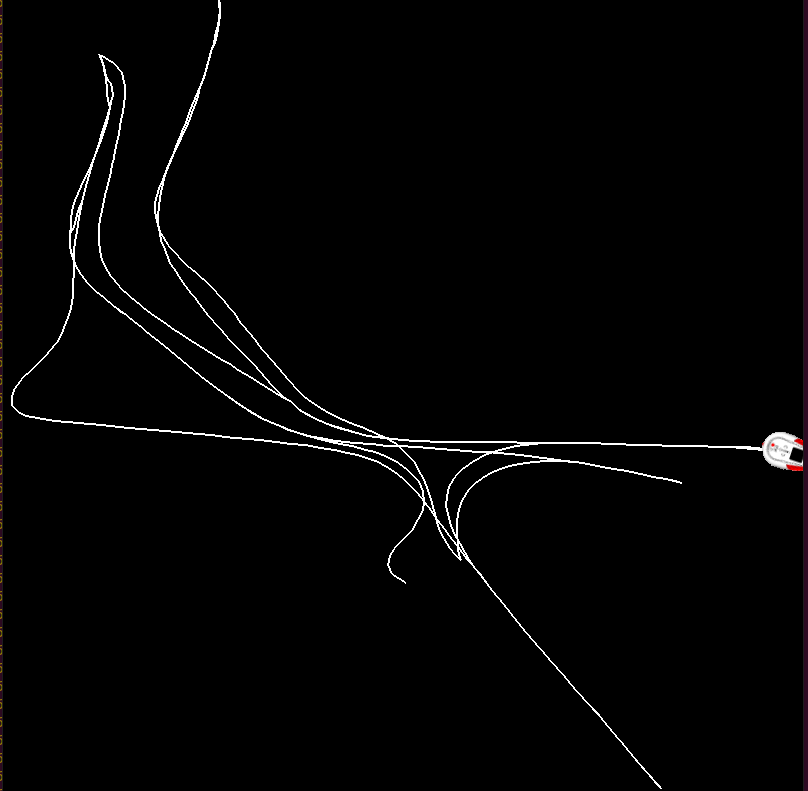
\includegraphics[height=0.3\textheight]{house-ratslam.png}\label{fig:mapsHouseRat}}
    \hfill
    \subfloat[Exact trajectory]{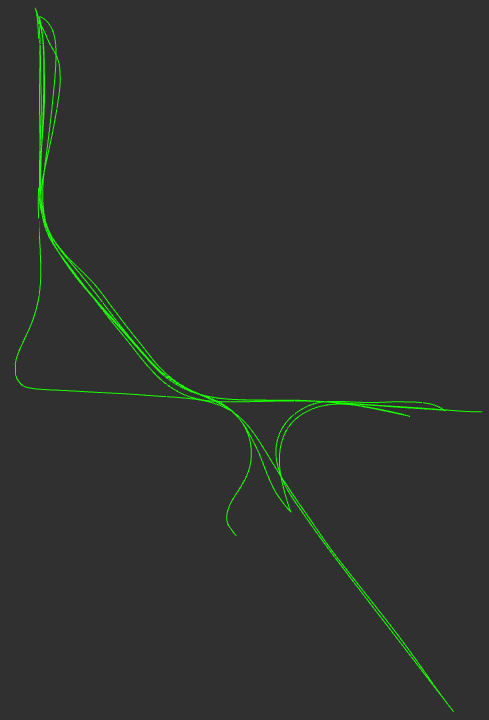
\includegraphics[height=0.3\textheight]{house-exact.png}\label{fig:mapsHouseEx}}
    \caption{Generated experience maps in the house environment}
    \label{fig:mapsHouse}
\end{figure}

\begin{figure}[!tbp]
    \centering
    \subfloat[1st Stage only approaches]{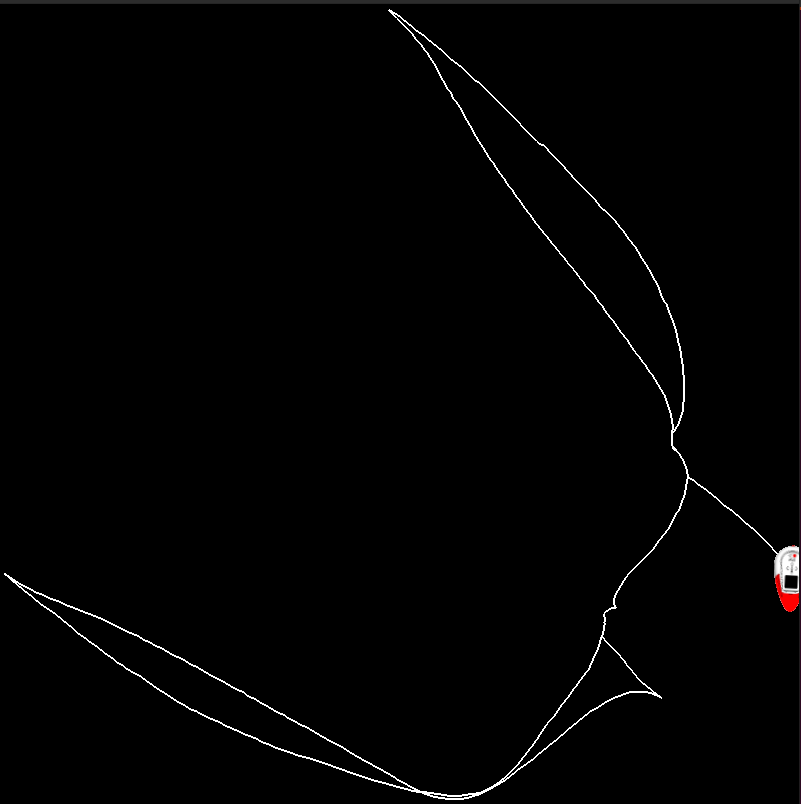
\includegraphics[height=0.3\textheight]{hospital-1stStage.png}\label{fig:mapsHospital1st}}
    \hfill
    \subfloat[Both stages approaches]{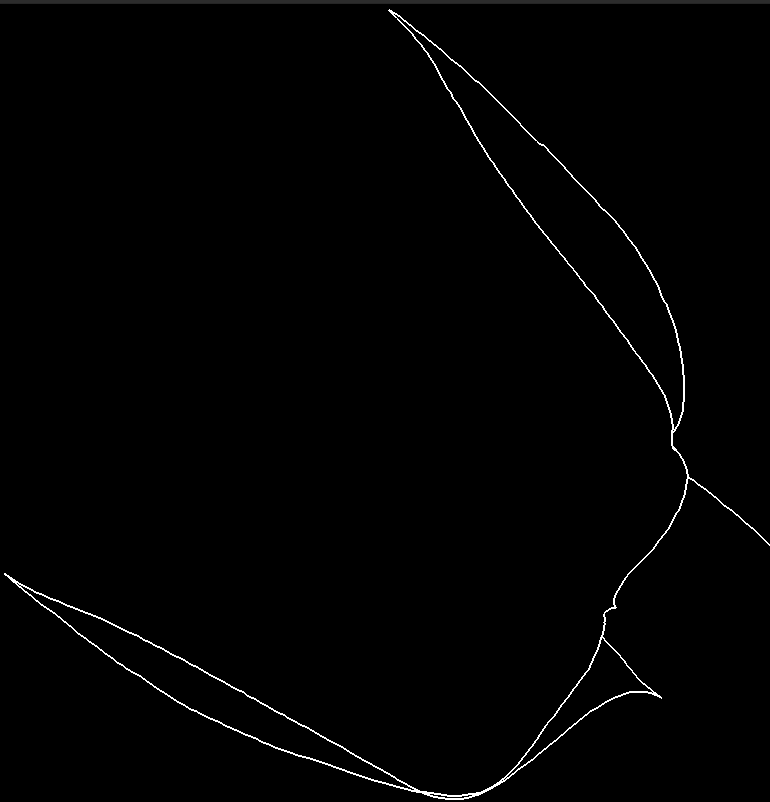
\includegraphics[height=0.3\textheight]{hospital-bothStages.png}\label{fig:mapsHospitalBot}}
    \\
    \subfloat[OpenRatSLAM]{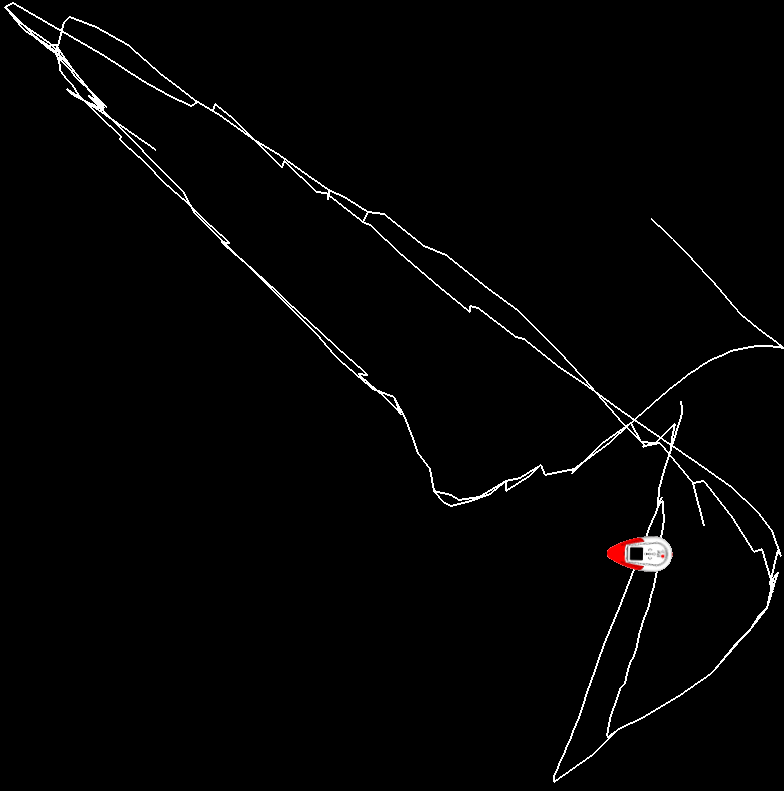
\includegraphics[height=0.3\textheight]{hospital-ratslam.png}\label{fig:mapsHospitalRat}}
    \hfill
    \subfloat[Exact trajectory]{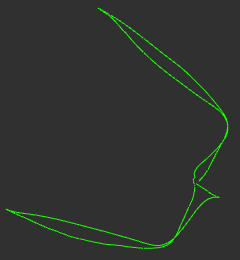
\includegraphics[height=0.3\textheight]{hospital-exact.png}\label{fig:mapsHospitalEx}}
    \caption{Generated experience maps in the hospital environment}
    \label{fig:mapsHospital}
\end{figure}

Figures \ref{fig:mapsWarehouse}, \ref{fig:mapsHouse}, and \ref{fig:mapsHospital} show the generated experience maps by every approach, including the OpenRatSLAM, together with the exact trajectory. The pictures clearly show that the results generated by the approaches with only the first stage and with both stages are almost identical. Even if the accuracy of the 2-stage approach was slightly better, the difference was too small to influence the results of the RatSLAM algorithm significantly. However, after comparing the generated maps with the exact trajectory, we can see that the results are satisfactory and that the suggested approaches are fully compatible with the RatSLAM algorithm.\par
Furthermore, the results from the hospital environment presented in Figure \ref{fig:mapsHospital} clearly show that the suggested approaches can outperform the OpenRatSLAM even in the generated trajectories. Because of the symmetry of the environment, the false evaluations of the visual scene recognition approach influenced the generated trajectory so significantly that it was entirely different from the exact one, and therefore, the OpenRatSLAM algorithm completely failed. However, the LiDAR sensors are considerably more precise in object distance estimation than a camera image, so the symmetry of the environment did not cause so many problems, and the generated results from the approaches suggested in this thesis were satisfactory.

\section{Discussion}\label{section:Discussion}

\chapter{Conclusion and Future Work}\label{chapter:conclusion}

In this thesis, the suitable scene representation and fusion of the data from LiDAR and camera sensors were performed. Afterward, two different approaches for the solution to scene recognition were suggested, and the whole system was integrated with the RatSLAM algorithm. Both proposed techniques operated smoothly during several experiments and significantly outperformed visual scene recognition and OpenRatSLAM. \par
The addition of a 3D LiDAR sensor to the camera proved beneficial. Not only were the results generated by the proposed methods more precise than those generated by OpenRatSLAM, but they also proved to work in environments where the OpenRatSLAM fails.

\section{Limitations}

Even if the approaches proved good performance in several experiments, there is still a possibility of unknown problems that may occur under several conditions.

\subsection*{Environments}

In this thesis, all simulations were performed in static environments. However, in praxis, the environments are rather dynamic and change over time, which might cause problems with scene recognition. Dynamic environments can also contain moving objects, which 3D LiDAR might poorly detect.\par
Furthermore, the approaches were optimized for indoor environments. In outdoor environments, the ground removal technique might fail because of rugged terrain. Outdoor scenes might also be empty or contain only very far objects, so the DBScan might detect zero clusters which can cause many false negative evaluations.

\subsection*{Sensors}

The addition of a LiDAR sensor to the system significantly lowers the sensors' frequency compared to the camera-only configuration. Even if this proved to not be a problem in section \ref{section:RatSalmIntegration}, it could still cause inaccuracies for mobile robots that move with a significantly higher speed than the TurtleBot used for the simulation.\par
Furthermore, the system was designed and tested with a LiDAR producing relatively sparse point clouds. In the case of usage of some higher quality alternatives, like depth cameras, producing significantly denser point clouds, the system can suffer from performance issues. However, applying any known downsampling technique before starting the fusion can quickly solve this problem.

\section{Future Work}

The neural system of humans or other mammals is still not wholly inspected and is still a prominent research topic. Therefore, there could come many new discoveries that can serve as an inspiration for the improvement of the RatSLAM or any other biologically inspired SLAM system. For example, the spike cells \cite{SpikeNN} represent a more accurate model of mammal neural cells and could be effectively used in the RatSLAM's grid network.\par
Different kinds of neural networks could also be tested for the second stage of the 2-stage approach. For example, HTM \cite{HTM} proved interesting results in combination with RatSLAM. Furthermore, the PointNet network, used as a feature extractor for the siamese network, can be trained on more suitable datasets. Because of the time constraints and limited offer of publicly available datasets, the network in this work was trained on a dataset containing only single objects instead of whole scenes. Even if this approach proved satisfactory, the more suitable training datasets might also improve the final accuracy of the results.\par
There are also additional sensors that could further improve the final results in combination with other sensors, like Dynamic Vision Sensors that can improve scene detection with moving objects. The used camera and LiDAR also have a limited field of view. Unlimited scenes could be detected using a panoramic camera and 360° 3D LiDAR. In this case, the scene recognition algorithm could also calculate a relative deviation between two differently rotated locations, which could positively influence the SLAM algorithm. Finally, these additional sensors can also be used to improve the accuracy of the odometry together with the scene recognition.\par
The color model could also be improved. For example, the Lab sphere can be divided into several sectors. The color would be represented as the id of the sector on the sphere instead of the exact Lab value. Instead of applying the CIE formula, the differences between sectors could be tabulated. This could save computational time and some memory and improve the algorithm's robustness against different light conditions.


% \appendix{}
% \chapter{General Addenda}

If there are several additions you want to add, but they do not fit into the thesis itself, they belong here.

\section{Detailed Addition}

Even sections are possible, but usually only used for several elements in, e.g.\ tables, images, etc.

\chapter{Figures}
\section{Example 1}
\cmark
\section{Example 2}
\xmark

\microtypesetup{protrusion=false}
\listoffigures{}
\listoftables{}
\microtypesetup{protrusion=true}
% \printglossaries
\printbibliography{}

\end{document}
